\documentclass[12pt]{article}

% ===== PACKAGES =====
\usepackage[a4paper,margin=2.7cm]{geometry}
\usepackage[utf8]{inputenc}
\usepackage[T1]{fontenc}
\usepackage{lmodern}

\usepackage{graphicx}
\usepackage{subcaption}
\usepackage{float}

\usepackage{amsmath, amssymb, amsfonts}
\usepackage{bm}

\usepackage{booktabs}
\usepackage{tabularx}
\usepackage{multirow}
\usepackage{array}

\usepackage{xcolor}
\usepackage{enumitem}

\usepackage{url}
\usepackage{hyperref}
\hypersetup{colorlinks=true, linkcolor=black, citecolor=black, urlcolor=blue}

\usepackage{caption}
\captionsetup{font=small, labelfont=bf}

\usepackage{cite}
\usepackage{setspace}
\onehalfspacing

\setlength{\parindent}{0pt}
\setlength{\parskip}{0.6em}

\newcommand{\R}{\mathbb{R}}
\newcommand{\E}{\mathbb{E}}

\begin{document}

\newcommand{\reporttitle}{Human-Robot Collaboration through VLA-based Learning}
\newcommand{\reportauthor}{Saniya Patwardhan}
\newcommand{\reporttype}{MRes Final Dissertation}
\newcommand{\cid}{06059013}
\date{\today}

\begin{titlepage}

\newcommand{\HRule}{\rule{\linewidth}{0.5mm}}


\includegraphics[width = 4cm]{figures/imperial}\\[0.5cm]

\begin{center}

\textsc{\LARGE \reporttype}\\[1.5cm]
\textsc{\Large Imperial College London}\\[0.5cm]
\textsc{\large Dyson School of Design Engineering}\\[0.5cm]

\HRule \\[0.4cm]
{ \huge \bfseries \reporttitle}\\
\HRule \\[1.5cm]
\end{center}

\begin{flushleft} \large
\textit{Author:}\\
\reportauthor~(CID: \cid)
\end{flushleft}
\vspace{1cm}
\textit{Research Supervisor:}\\
Assoc. Prof. Petar Kormushev

\vspace{1cm}
\makeatletter
Date: \@date

\vspace{4cm}
\begin{center}
    I confirm that this report is my own original work and has
not been copied or submitted elsewhere. Any use of AI tools has been appropriately acknowledged and
has not replaced my own intellectual contribution. All sources have been properly referenced.
\end{center}

\vfill

\makeatother

\end{titlepage}


\title{Human-Robot Collaboration through VLA-based Learning}
\author{Saniya Patwardhan \\ Dyson School of Design Engineering, Imperial College London}
\maketitle

\begin{abstract}
Human--robot collaboration (HRC) requires robots that can understand high-level goals, adapt to novel embodiments, and act reliably alongside people. Vision--Language--Action (VLA) models promise an end-to-end route to this by mapping visual observations and language instructions directly to robot actions, but adapting a pretrained VLA to a new robot, and combining it with high-level task reasoning, remains poorly understood.

This dissertation reports the full arc of an MRes project that adapts the $\pi$0.5 VLA model to a Baxter-based collaborative manipulation system. Building on an early-stage exploration of vision--language monitoring and a late-stage LoRA fine-tuning and inference pipeline, this final stage contributes three further lines of evidence: (i) an extension of the fine-tuning pipeline to two additional embodiments (Franka Emika Panda and Unitree G1) to study cross-embodiment skill transfer, (ii) a Vision--Language Model (VLM) planner, now described and evaluated in detail, that decomposes goal-directed rearrangement into primitive instructions and closes the loop with a goal-check--replan cycle, together with an evaluation protocol for the resulting human--robot collective task, and (iii) validation of the fine-tuned policy on a physical Baxter robot.

Consistent with the late-stage findings, transitioning the manipulation policy from velocity-control to position-control actions, and maintaining strict train--inference consistency, were the dominant levers on manipulation performance, improving trial-level success from 0\% to 43\% across six pick-and-place tasks. The cross-embodiment extension yielded 128 and 113 success-filtered demonstration episodes for Franka and G1 respectively, exposing embodiment-specific reach and gripper-force constraints, with joint multi-embodiment training and solo-versus-joint comparison identified as the immediate next step. The VLM planner's per-block, constrained-format prompting strategy is shown to resolve the structured-output unreliability identified during the early stage of the project. Physical deployment infrastructure connecting a ROS-driven remote controller to a GPU policy server over a websocket, with a locally attached RealSense camera supplying the scene view, is described and readied for single-block validation trials.

Project updates, demonstrations, and source code are available at \texttt{https://saniya2912.github.io/pi05-baxter/}.
\end{abstract}

\clearpage

% =====================================================================
\section{Introduction}
\label{sec:intro}

Humans and robots have complementary strengths: robots offer precision and repeatability, while humans offer dexterity, judgement, and adaptability in unstructured settings. Realising human--robot collaboration (HRC) that exploits both requires a robot that can (i) understand a high-level, often loosely specified goal, (ii) translate that goal into a sequence of physically executable actions, and (iii) carry out those actions reliably on real hardware, ideally while remaining responsive to a human partner who may change the task mid-way. Traditional robotic systems, built around predefined workflows and isolated perception, planning, and control modules, struggle to meet all three requirements simultaneously.

Vision--Language--Action (VLA) models offer a promising route to this goal by learning a direct mapping from visual observations and natural-language instructions to robot actions, rather than hand-engineering separate perception and control stages. Models such as RT-1, RT-2, OpenVLA, and the $\pi$0/$\pi$0.5 family have demonstrated that large-scale multimodal pretraining can produce policies with meaningful language grounding and some transfer across tasks and robots. However, two problems remain underexplored. First, adapting a VLA model pretrained on other embodiments to a genuinely new robot -- with its own kinematics, camera placement, and control interface -- is not a solved problem, and the specific engineering decisions involved (action representation, demonstration quality, train--inference consistency) have received little systematic study. Second, VLA models are action-centric: they do not by themselves reason about high-level task structure, multi-step goals, or a human partner's intent, which motivates pairing them with a higher-level planning layer.

This project addresses both problems by adapting the $\pi$0.5 VLA model to a Baxter robot in a custom MuJoCo pick-and-place environment, and by pairing the fine-tuned policy with a Vision--Language Model (VLM) planner that converts a goal image into an ordered sequence of manipulation instructions. The project has proceeded in three stages, each captured in a gateway report, with this dissertation consolidating and extending all of them.

The \emph{early stage} established the motivation and explored the individual system components in isolation: a hybrid VLM+VLA architecture was proposed, in which a vision--language model would decompose a natural-language goal into verifiable subtasks and monitor human progress towards them, while a VLA policy executed subtasks assigned to the robot. Preliminary experiments compared a detection-based approach (GroundingDINO) against a purely vision--language approach (Gemma-3-12B) for monitoring object arrangements, and a first, unmodified deployment of $\pi$0.5 -- pretrained on a 7-DOF Franka robot via the LIBERO benchmark -- onto a simulated 15-DOF Baxter exposed fundamental mismatches in action space, state representation, and gripper control. This zero-shot failure, rather than being a setback, directly motivated the fine-tuning programme that followed: it demonstrated that direct transfer of a pretrained VLA policy to a new embodiment is insufficient, and that either task-specific fine-tuning or an intermediate kinematic mapping is required.

The \emph{late stage} developed that fine-tuning programme in full: a scripted, inverse-kinematics-based demonstration collection pipeline; a Low-Rank Adaptation (LoRA) fine-tuning framework built on the OpenPI training stack; a two-process websocket inference architecture; and a first working version of the Gemma-3-12B VLM planner. Systematic checkpoint comparisons identified that the choice of action representation (velocity- versus position-control) and the elimination of train--inference mismatches, rather than additional training steps or lower training loss, were the dominant factors governing manipulation success.

This \emph{final stage}, reported here, extends the work along the three axes identified as the natural continuation of that programme. First, the fine-tuning and demonstration-collection pipeline is extended from Baxter alone to two further embodiments, Franka Emika Panda and Unitree G1, to study whether a single policy trained jointly across embodiments transfers skill positively or negatively relative to three independently fine-tuned solo policies -- a direct empirical test of the cross-embodiment generalisation that pretrained VLA models such as $\pi$0.5 claim, but rarely verify at the fine-tuning stage. Second, the VLM planner, previously reported only as a single-page component, is described here in full engineering detail, including the per-block prompting strategy that resolves the structured-output unreliability identified during the early stage, and its closed-loop goal-check--replan cycle; an evaluation protocol for the full human--robot \emph{collective task} -- in which the robot and a human jointly rearrange a shared workspace, with the human able to modify the scene mid-execution -- is defined and readied for evaluation. Third, the fine-tuned policy and its inference stack are deployed towards validation on a physical Baxter robot, with the scene camera attached directly to the policy-serving machine and joint state and wrist imagery relayed over ROS and a websocket from a separate control laptop; a single-block pick-and-place trial is the first physical validation milestone.

Beyond the specific research questions this project answers, the work is motivated by a practical deployment target: Robot DE NIRO, a human-centred, dual-arm mobile research platform built around a Baxter upper body and developed specifically to support cognitively-enhanced manipulation research in shared human workspaces. Every methodological choice made in this project -- the Baxter-based simulation environment, the choice of a fine-tunable rather than a from-scratch policy, the six-primitive task decomposition, and, in this final stage, the extension to further embodiments and to physical hardware -- was made with an eye to whether it would still make sense once the system left simulation and was asked to operate autonomously on DE NIRO's own arms, or on a robot with a different arm entirely. This is also why cross-embodiment generalisation (RQ4) is treated as a first-class research question in this final stage rather than an afterthought: a collaboration framework that only works for the exact Baxter simulation it was developed in would be a considerably weaker contribution than one shown to extend, with modest additional engineering effort, to other manipulator geometries.

The remainder of this dissertation is structured as follows. Section~\ref{sec:litrev} reviews related work in human--robot collaboration and Vision--Language--Action models. Section~\ref{sec:gap} identifies the resulting research gap and states the research questions this dissertation answers. Section~\ref{sec:methodology} describes the complete methodology, from the original Baxter pipeline through to the three new lines of work. Section~\ref{sec:results} reports results, distinguishing between the mature simulation-policy findings and the newer experiments, which are reported as evaluation protocols with data collected so far, pending full completion. Section~\ref{sec:discussion} critically reflects on the project as a whole, and Section~\ref{sec:conclusion} concludes and outlines the work remaining before submission.

% =====================================================================
\section{Literature Review}
\label{sec:litrev}

\subsection{Human--Robot Collaboration}

Human--robot collaboration (HRC) aims to enable humans and robots to work together by leveraging their complementary capabilities \cite{ajoudani2018progress}. The emergence of collaborative robots (cobots) has enabled safe operation in shared workspaces without the physical barriers required by traditional industrial robots \cite{robotics8040100}. While these systems have improved physical co-location and coordination, many still rely on separate perception, planning, and control modules and do not explicitly reason about subtask-level allocation of roles between human and robot partners, limiting their ability to adapt to changing task goals \cite{gervasi2020conceptual}. A conceptual framework for evaluating human-robot collaboration further distinguishes coordination quality from raw task throughput, arguing that collaboration should be assessed by how well the human and robot jointly adapt to each other's actions rather than by task completion time alone \cite{gervasi2020conceptual} -- a distinction directly relevant to this dissertation's collaborative task success metric (Section~\ref{sec:methodology-hrc}), which likewise separates primitive-level execution quality from whether the overall human--robot exchange, including the robot's response to a human-initiated change, was completed correctly.

Recent work has addressed different aspects of collaborative reasoning. SAGE combines action and gaze estimation to capture fine-grained human behaviour for comprehensive human behaviour analysis \cite{kuang2025sage}, while Therblig-based methods represent manipulation as structured action primitives, drawing on classical motion-study taxonomies to describe human and robot actions in a shared vocabulary \cite{reinhardt2024therblig}. Long-horizon planning approaches decompose complex tasks into sequences of executable primitives that a backbone model can reason over \cite{Chen_2025}. Visual instruction understanding has also been demonstrated on LEGO-assembly benchmarks, where a visual manual is translated into a machine-executable plan \cite{wang2022translating}, or where interactive structural understanding is used to break and make LEGO structures from images \cite{walsman2022break}. Although effective, these methods typically depend on handcrafted task representations or specialised pipelines, which limits their generalisation to new domains and object sets.

\subsection{Vision--Language--Action Models}

Prior to the emergence of Vision--Language--Action (VLA) models, systems such as SayCan combined large language models with predefined robotic skill libraries for language-guided planning \cite{ahn2022icanisay}. While effective for structured tasks, they relied on manually designed skill libraries rather than end-to-end visuomotor learning, so the set of achievable behaviours was fixed by the skill library rather than learned from demonstration.

Recent VLA models instead learn a direct mapping from visual observations and language instructions to robot actions. RT-1 demonstrated large-scale robotic learning from real-world data \cite{brohan2023rt1roboticstransformerrealworld}, while RT-2 incorporated vision--language pretraining on web-scale data to improve semantic reasoning and generalisation to novel objects and instructions \cite{brohan2023rt2visionlanguageactionmodelstransfer}. Open-source models such as OpenVLA \cite{kim2024openvlaopensourcevisionlanguageactionmodel} and SmolVLA \cite{shukor2025smolvlavisionlanguageactionmodelaffordable} have made VLA research more broadly accessible, while the $\pi$0 and $\pi$0.5 models introduce flow matching to predict chunks of future actions rather than single-step commands, improving the smoothness and coherence of continuous manipulation \cite{black2026pi0visionlanguageactionflowmodel, intelligence2025pi05visionlanguageactionmodelopenworld}. Notably, $\pi$0.5 is explicitly trained jointly across a heterogeneous set of embodiments (including ALOHA, DROID, and Bridge-style platforms) via action-dimension padding, which the model's authors present as evidence of open-world generalisation. However, this joint-embodiment property is evaluated at the pretraining scale, and it remains unclear whether it holds -- or whether embodiments interfere with one another -- when a small, task-specific dataset is used to \emph{fine-tune} the model on a new set of embodiments simultaneously, rather than pretrain it from scratch. This is precisely the question the cross-embodiment extension in this dissertation investigates empirically. A recent survey situates these developments and highlights the gap between VLA research, which is overwhelmingly policy-centric, and the requirements of real-world deployment, including adaptation to new embodiments \cite{11164279}. Reinforcement-fine-tuning approaches such as VLA-RFT further suggest that verified reward signals from world simulators can refine VLA behaviour beyond imitation learning alone, an avenue not explored in this project but relevant to future refinement of the fine-tuned policy \cite{li2025vla}. Most VLA research, however, continues to focus on policy learning in isolation, rather than on adaptation to new robot embodiments or integration with high-level, goal-directed planning -- the combination this project targets.

It is worth situating this VLA-centric line of work against the classical imitation-learning literature it builds on. Earlier multimodal-integration approaches to manipulation learning already demonstrated that combining vision, proprioception, and other sensory modalities in a shared representation improves skill acquisition \cite{NODA2014721}, and multi-sensor encoding schemes were developed specifically to support learning from multimodal demonstration of this kind \cite{zeng2019encoding}. What VLA models such as $\pi$0.5 add on top of this established multimodal-imitation-learning foundation is, first, a natural-language rather than a purely visual task specification, allowing a single policy to be conditioned on an open vocabulary of instructions rather than a fixed set of demonstrated behaviours, and second, a large-scale pretraining corpus spanning many robots and tasks, intended to provide transferable priors rather than requiring every new task to be learned from that task's demonstrations alone. The zero-shot baseline result reported in Section~\ref{sec:results-sim} (a non-trivial 15\% success rate on an entirely unseen Baxter embodiment) is direct evidence that this pretraining transfer is real, if partial, and it is this partial-but-real transfer -- rather than either complete failure or complete success -- that motivates fine-tuning as the appropriate intervention, and motivates asking, as this dissertation's cross-embodiment extension does, how much of that transfer is retained or lost when a single small-scale fine-tuning run is asked to cover several embodiments at once.

\subsection{Language as an Interface for Collaboration}

Natural language has become an important interface for human--robot interaction. Wang~\emph{et al.} proposed a framework for modifying robot trajectories through language, allowing a user to adjust a robot's planned position, velocity, or force in real time using natural-language commands interpreted by a large language model \cite{wang2026bidirectionalhumanrobotcommunicationphysical}. This approach, however, focuses on low-level modification of trajectories that are predefined rather than generated after context-aware task planning. VLA-bot combines multimodal perception with manipulation for collaborative assembly tasks, requesting human assistance through an augmented-reality interface for long-horizon tasks \cite{WANG2026103268}, but does not explicitly monitor human-performed subtasks or their role in dynamic task allocation, and its VLA component is a custom framework mapping human verbal and visual input to motion sequences rather than a large pretrained VLA model, which may limit its generalisability. Neither of these works investigates efficient adaptation of large pretrained VLA models to novel robotic platforms while also closing the loop with high-level, image-conditioned planning, which is the combination pursued here.

\subsection{Multimodal Learning for Manipulation and Platform Context}

Earlier work on multimodal integration for robot behaviour learning demonstrated that combining multiple sensory modalities in a shared representation improves manipulation skill acquisition \cite{NODA2014721}, and encoding schemes for multi-sensor demonstration data have been proposed to support this style of learning from multimodal demonstration \cite{zeng2019encoding}. The Robot DE NIRO platform, a human-centred, autonomous, mobile research platform built around a dual-arm Baxter manipulator, was developed specifically to support cognitively-enhanced manipulation and human-centred robotics research of this kind \cite{falck2020robot, falck2018human}, and motivates the choice of a Baxter-based system as the target embodiment for this project, since it provides a direct route to eventual deployment on DE NIRO.

\subsection{Summary and Positioning}

Overall, recent advances in multimodal robotics have significantly improved robot perception, planning, and manipulation individually, but three gaps persist at their intersection. First, systematic study of adapting pretrained VLA models to novel embodiments with different kinematics, camera viewpoints, and control interfaces -- and of whether a single model can be fine-tuned jointly across several such embodiments without negative transfer -- remains limited. Second, hierarchical frameworks that integrate a VLM planner with a fine-tuned VLA policy, and that close the loop by re-planning in response to a dynamically changing, human-modified scene, are rarely demonstrated end-to-end. Third, limited attention has been given to the engineering decisions -- action representation, demonstration generation, and train--inference consistency -- that determine whether VLA adaptation succeeds at all, and to validating the resulting policies on physical hardware rather than only in simulation. This dissertation addresses all three gaps directly: the first through the cross-embodiment extension to Franka and G1 (Section~\ref{sec:methodology-crossemb}), the second through the VLM planner's closed-loop goal-check--replan cycle and the collective-task evaluation protocol built on it (Sections~\ref{sec:vlm-planner}--\ref{sec:methodology-hrc}), and the third through the systematic checkpoint comparison and train--inference mismatch analysis carried over from the late stage (Section~\ref{sec:results-sim}) together with the physical deployment architecture reported in Section~\ref{sec:methodology-realrobot}.

% =====================================================================
\section{Research Gap and Questions}
\label{sec:gap}

\subsection{Research Gap}

Despite recent advances in Vision--Language--Action (VLA) models, five gaps motivate this dissertation. First, efficient adaptation of pretrained VLA models to novel robot embodiments with different kinematics, camera viewpoints, and control interfaces remains underexplored, and it is unclear whether a single model can be fine-tuned jointly across multiple new embodiments without embodiments interfering with one another. Second, high-level task planning and low-level manipulation are typically addressed separately, with few hierarchical frameworks integrating Vision--Language Models (VLMs) and VLA policies, and fewer still that close the loop with re-planning when a human modifies the scene. Third, limited attention has been given to the engineering decisions that influence VLA adaptation, including action representation, demonstration generation, and train--inference consistency. Fourth, VLM-based reasoning layers are known to produce unreliable structured outputs when asked to reason about multiple objects simultaneously, which limits their direct use for task monitoring or planning unless the prompting strategy is specifically designed around this weakness. Fifth, the great majority of VLA adaptation work, including the early and late stages of this project, is validated only in simulation, leaving open whether the resulting policies transfer to physical hardware.

\subsection{Research Questions}

This dissertation is guided by the following research questions, the first three of which were established during the earlier stages of the project and are answered in full here, and the remaining three of which define the new contributions of this final stage.

\begin{enumerate}
\item[\textbf{RQ1}] How effectively can a pretrained Vision--Language--Action model be adapted to a novel robot embodiment?
\item[\textbf{RQ2}] How do engineering decisions, including action representation, demonstration generation, and train--inference consistency, affect manipulation performance?
\item[\textbf{RQ3}] Can a Vision--Language Model be integrated with a fine-tuned Vision--Language--Action policy to achieve goal-directed manipulation, including closed-loop re-planning when the workspace changes?
\item[\textbf{RQ4}] Does jointly fine-tuning a single VLA policy across multiple robot embodiments (Baxter, Franka, and G1) produce positive skill transfer relative to independently fine-tuned, single-embodiment policies, or does it degrade performance through negative transfer?
\item[\textbf{RQ5}] Can the integrated planner--policy system complete a human--robot \emph{collective task}, in which the robot and a human jointly rearrange a shared workspace and the human is free to modify the scene mid-execution, and how is collaborative task success best measured?
\item[\textbf{RQ6}] Does a policy fine-tuned and validated in simulation transfer to a physical Baxter robot, and what does the sim-to-real gap reveal about the adequacy of the simulation environment?
\end{enumerate}

% =====================================================================
\section{Methodology}
\label{sec:methodology}

\subsection{Overall System Architecture}

The proposed framework (Fig.~\ref{fig:architecture}) follows a hierarchical architecture consisting of a Vision--Language Model (VLM) planner and a Vision--Language--Action (VLA) policy. The Gemma-3-12B VLM compares the current and goal workspace images to generate an ordered sequence of manipulation primitives. Each primitive is provided as a language instruction to a fine-tuned $\pi$0.5 policy, which generates robot actions from visual observations and robot state information. Separating planning from execution enables independent evaluation of each component and supports re-planning when the workspace changes, whether due to policy execution error or deliberate human intervention.

\begin{figure}[H]
\centering
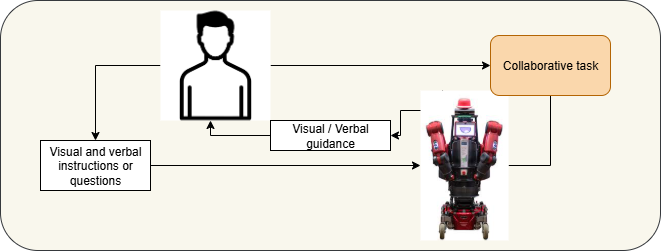
\includegraphics[width=0.85\linewidth]{figures/late_stage_images/hrc.png}
\caption{Proposed hierarchical system architecture: a human specifies a goal, the VLM planner converts the current/goal image pair into an ordered task list, and the fine-tuned $\pi$0.5 policy executes each primitive in the target environment (MuJoCo simulation or physical Baxter).}
\label{fig:architecture}
\end{figure}

\subsection{Design Engineering Approach}
\label{sec:design-approach}

Being conducted within the Dyson School of Design Engineering, this project followed a structured design process rather than a single-pass research pipeline, and this process is itself worth documenting since it shaped several of the decisions described later in this section.

Two design-engineering framings, both introduced at the early-stage gateway, remained in use throughout. The first is systematic inventive thinking applied to a resource-constrained problem: training a full Vision--Language--Action system from scratch was recognised early as impractical given the computational budget available, so the problem was instead decomposed into modular components built from pretrained models -- a VLM for high-level reasoning, a VLA for low-level control -- combined rather than trained end-to-end. This decomposition, chosen for tractability, turned out to have a second benefit that only became apparent later: because the VLM planner and the VLA policy are independently swappable modules communicating through a fixed language-instruction interface, extending the system to two further robot embodiments (Section~\ref{sec:methodology-crossemb}) required no change whatsoever to the planner, and extending it to physical hardware (Section~\ref{sec:methodology-realrobot}) required no change to the policy's training procedure -- only to the client supplying its observations.

The second framing is a Double Diamond process applied at the project level: the project began with the broad goal of enabling human-centred robotic assistance, explored multiple candidate architectures (including a detection-based monitoring pipeline using GroundingDINO, and a free-form VLM-based monitoring pipeline, both described in Section~\ref{sec:early-monitoring}) before converging on the VLM-planner-plus-VLA-policy architecture used throughout the late and final stages, and is now, in this final stage, diverging again -- deliberately -- into three parallel extensions (cross-embodiment, collaborative task, physical deployment) of that converged architecture, each probing a different dimension of its generality.

At the level of individual components, the project followed an iterative engineering design process in which experimental findings continuously informed subsequent development, rather than implementing the complete collaborative framework in a single stage. Individual components -- the simulation environment, the demonstration-collection pipeline, the fine-tuned policy, and the VLM planner -- were developed, evaluated, and refined independently before integration, and each was validated in isolation before being combined with the others. Key engineering contributions produced by this process include the custom MuJoCo simulation environment; the scripted Damped Least Squares inverse-kinematics data-collection pipeline (Section~\ref{sec:demo-pipeline}); the LoRA-based adaptation of the $\pi$0.5 Vision-Language-Action model; the redesign of the action representation from velocity to position control (Section~\ref{sec:action-rep}); and the hierarchical Vision-Language planner for task sequencing (Section~\ref{sec:vlm-planner}). This incremental development strategy reduced hardware risk, enabled rapid experimentation, and allowed individual design decisions to be evaluated systematically before progressing towards end-to-end human-robot collaboration -- and the same strategy was re-applied, largely unchanged, to stage each of this final stage's three extensions independently (Sections~\ref{sec:methodology-crossemb}--\ref{sec:methodology-realrobot}) before any attempt to combine them.

\subsection{Choice of Platform}

\subsubsection{Robot DE NIRO and Baxter}
Robot DE NIRO was selected as the long-term deployment platform due to its Baxter-based dual-arm configuration, mobile base, and human-centred design, making it well suited to human--robot collaboration research \cite{falck2020robot}. Development in the late stage focused on simulation; this final stage additionally targets a physical Baxter robot directly (Section~\ref{sec:methodology-realrobot}), sharing the same 7-DOF right-arm kinematics and Rethink parallel-jaw gripper as DE NIRO's upper body, so that the fine-tuned policy and inference stack transfer without modification to the DE NIRO platform in future work.

\begin{figure}[H]
\centering
\begin{subfigure}[b]{0.44\linewidth}
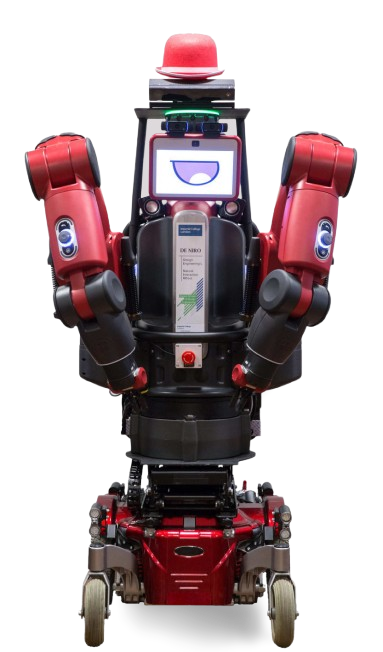
\includegraphics[width=\linewidth]{figures/late_stage_images/De_Niro.png}
\caption{Robot DE NIRO, the long-term target platform.}
\end{subfigure}
\hfill
\begin{subfigure}[b]{0.44\linewidth}
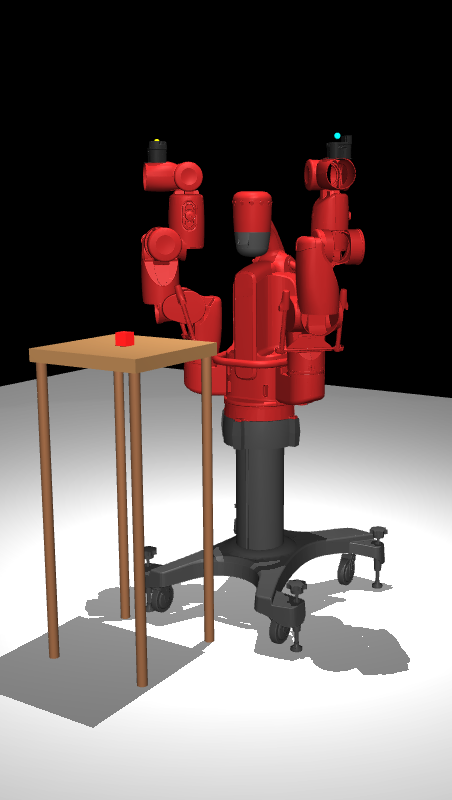
\includegraphics[width=\linewidth]{figures/late_stage_images/baxter_mujoco.png}
\caption{Baxter in the custom MuJoCo pick-and-place environment.}
\end{subfigure}
\caption{The physical DE NIRO platform and its simulated Baxter counterpart used throughout development.}
\label{fig:deniro_mujoco}
\end{figure}

\subsubsection{MuJoCo Simulation}
Development was performed primarily in the MuJoCo physics simulator to enable rapid experimentation, safe debugging, and automated demonstration collection. Simulation also allowed train--inference mismatches to be identified and resolved before deployment, and provided a reliable environment for policy development, checkpoint evaluation, and -- in this final stage -- the construction of Franka and G1 variants of the same tabletop environment for the cross-embodiment extension. MuJoCo specifically, rather than an alternative simulator, was retained from the early stage of the project primarily for continuity and for its offscreen rendering support, which the demonstration-collection pipeline's dual-camera observations (Section~\ref{sec:demo-pipeline}) and the VLM planner's goal-image rendering (Section~\ref{sec:vlm-planner}) both depend on directly, and its native support for manufacturer MJCF assets, which made importing Franka's and G1's own mesh and kinematic descriptions in Section~\ref{sec:methodology-crossemb} a matter of asset conversion rather than re-modelling each robot from scratch.

\subsubsection{$\pi$0.5}
The $\pi$0.5 Vision-Language-Action (VLA) model released by Physical Intelligence was selected as the foundation policy for this research. The model combines visual observations, robot state information, and natural language instructions to generate robot actions directly from high-level task descriptions. Several factors motivated its selection. First, $\pi$0.5 has demonstrated strong manipulation performance across multiple robotic embodiments. Second, the model's release includes a training and inference framework (OpenPI) that can be adapted to custom robotic platforms. Finally, the model supports parameter-efficient fine-tuning, making experimentation feasible within the computational resources available for this project.

Compared to other open VLA models such as OpenVLA, $\pi$0.5 employs a flow-matching architecture that predicts action chunks rather than individual actions. This enables more expressive trajectory modelling and was considered particularly suitable for the sequential manipulation tasks investigated in this work. A comparison between the two approaches is shown in Table~\ref{tab:openvla_pi05}.

\begin{table}[H]
\centering
\caption{Comparison of OpenVLA and $\pi$0.5}
\label{tab:openvla_pi05}
\begin{tabular}{ll}
\toprule
\textbf{OpenVLA} & \textbf{$\pi$0.5} \\
\midrule
Open-source model & Research release \\
Autoregressive actions & Flow-matching actions \\
Single-step prediction & Action chunk prediction \\
Simpler training paradigm & Advanced trajectory modelling \\
Easier deployment & Stronger manipulation modelling \\
\bottomrule
\end{tabular}
\end{table}

\subsection{Early-Stage Monitoring Pilot}
\label{sec:early-monitoring}

Before committing to the VLM planner design described in Section~\ref{sec:vlm-planner}, the early stage of this project piloted two candidate approaches to visually monitoring a multi-object arrangement task: a detection-based approach using GroundingDINO, and a purely vision--language approach using a pretrained Gemma-3-12B model, on a real-world fruit-sorting task observed through a live RGB camera (Fig.~\ref{fig:early_monitoring}).

\begin{figure}[H]
\centering
\begin{subfigure}[b]{0.31\linewidth}
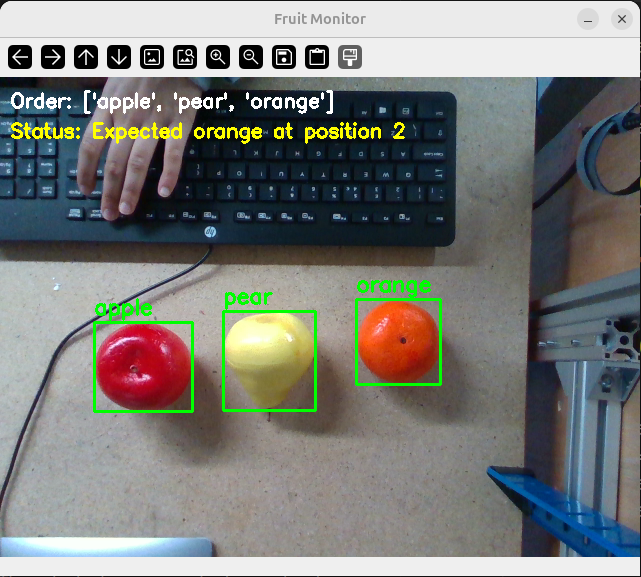
\includegraphics[width=\linewidth]{figures/late_stage_images/incomplete_task.png}
\caption{GroundingDINO: incorrect order detected.}
\end{subfigure}
\hfill
\begin{subfigure}[b]{0.31\linewidth}
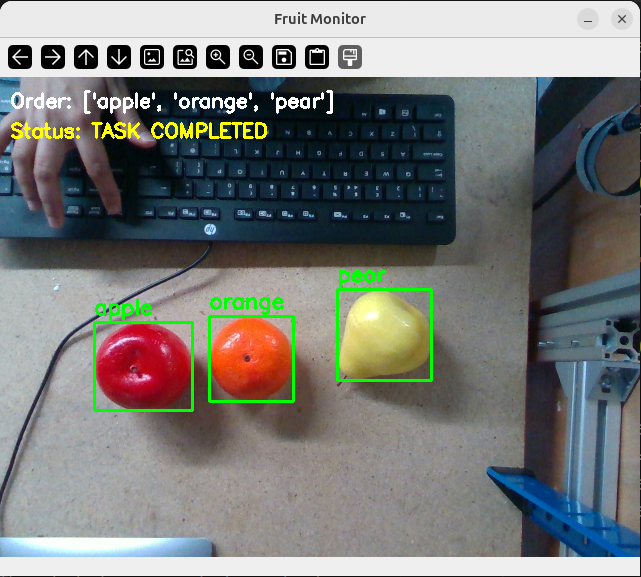
\includegraphics[width=\linewidth]{figures/late_stage_images/task_complete.png}
\caption{GroundingDINO: task completed.}
\end{subfigure}
\hfill
\begin{subfigure}[b]{0.31\linewidth}
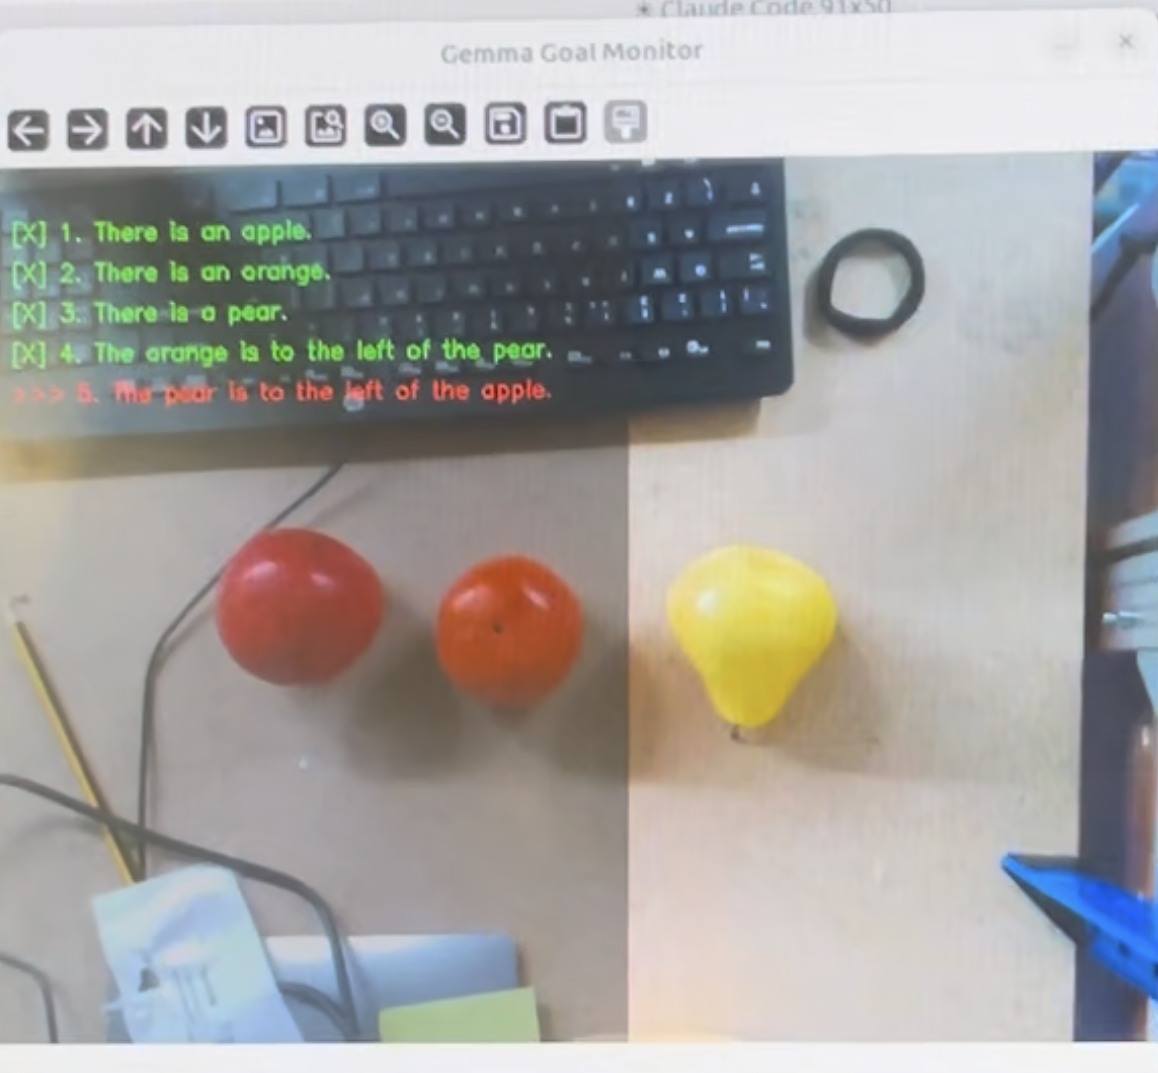
\includegraphics[width=\linewidth]{figures/late_stage_images/gemma_monitor.png}
\caption{Gemma-3-12B goal monitor: per-condition checklist, with a failed spatial-relation check shown in red.}
\end{subfigure}
\caption{Early-stage monitoring pilot on a real-world fruit-sorting task: detection-based (GroundingDINO) versus vision--language (Gemma-3-12B) monitoring of task progress.}
\label{fig:early_monitoring}
\end{figure}

GroundingDINO provided reliable, precisely localised object detections and could verify simple spatial relationships (e.g.\ left-to-right ordering) robustly, but required predefined object queries and had no capacity for higher-level task reasoning. Gemma-3-12B, conversely, produced accurate free-form natural-language scene descriptions and could reason flexibly about arbitrary goal conditions, but its structured, checklist-style output was materially less reliable, particularly once more than one spatial relationship had to be verified simultaneously (Fig.~\ref{fig:early_monitoring}c shows exactly this failure mode: the fourth condition is verified correctly, but the fifth, which depends jointly on two previously-mentioned objects, is not). This trade-off -- reliable detection with no reasoning versus flexible reasoning with unreliable structured output -- is the direct motivation for the per-block, single-object querying strategy adopted in the VLM planner described in Section~\ref{sec:vlm-planner}.

\subsection{Vision-Language-Action Adaptation Strategy}

\subsubsection{Need for Fine-Tuning}
Although Vision--Language--Action (VLA) models are pretrained on diverse robots and manipulation tasks, direct deployment on a new robot is challenging due to differences in kinematics, camera placement, workspace configuration, and control interfaces. This was confirmed empirically during the early stage of the project: the unmodified, zero-shot $\pi$0.5 policy -- originally trained on the LIBERO benchmark using a 7-DOF Franka robot -- was deployed without modification on the 15-DOF Baxter system in MuJoCo (Fig.~\ref{fig:deniro_mujoco}b). Diagnostic logging of this zero-shot rollout exposed three compounding mismatches. First, the policy's 7-dimensional end-effector action output (Fig.~\ref{fig:zeroshot_actions}) was naively mapped onto Baxter's joint-velocity space, so that only the right arm was actuated. Second, the policy expected an 8-dimensional end-effector state but instead received raw Baxter joint angles (Fig.~\ref{fig:zeroshot_diagnostics}) -- a semantically incorrect input, since, for example, the value the policy interpreted as a roll angle in radians was in fact the shoulder joint's raw position. Third, the policy re-plans a full action chunk every 10 steps regardless of scene change, and the resulting L2 norm of the commanded action (Fig.~\ref{fig:zeroshot_l2norm}) shows persistent, non-decaying step-changes rather than the settling behaviour expected as a manipulation task approaches completion. The gripper command was also ignored entirely due to the absence of a corresponding actuator mapping. The system was functionally integrated end-to-end, yet exhibited no meaningful task execution, confirming that direct transfer of a pretrained VLA policy is insufficient and that either task-specific fine-tuning or an intermediate kinematic mapping is required.

\begin{figure}[H]
\centering
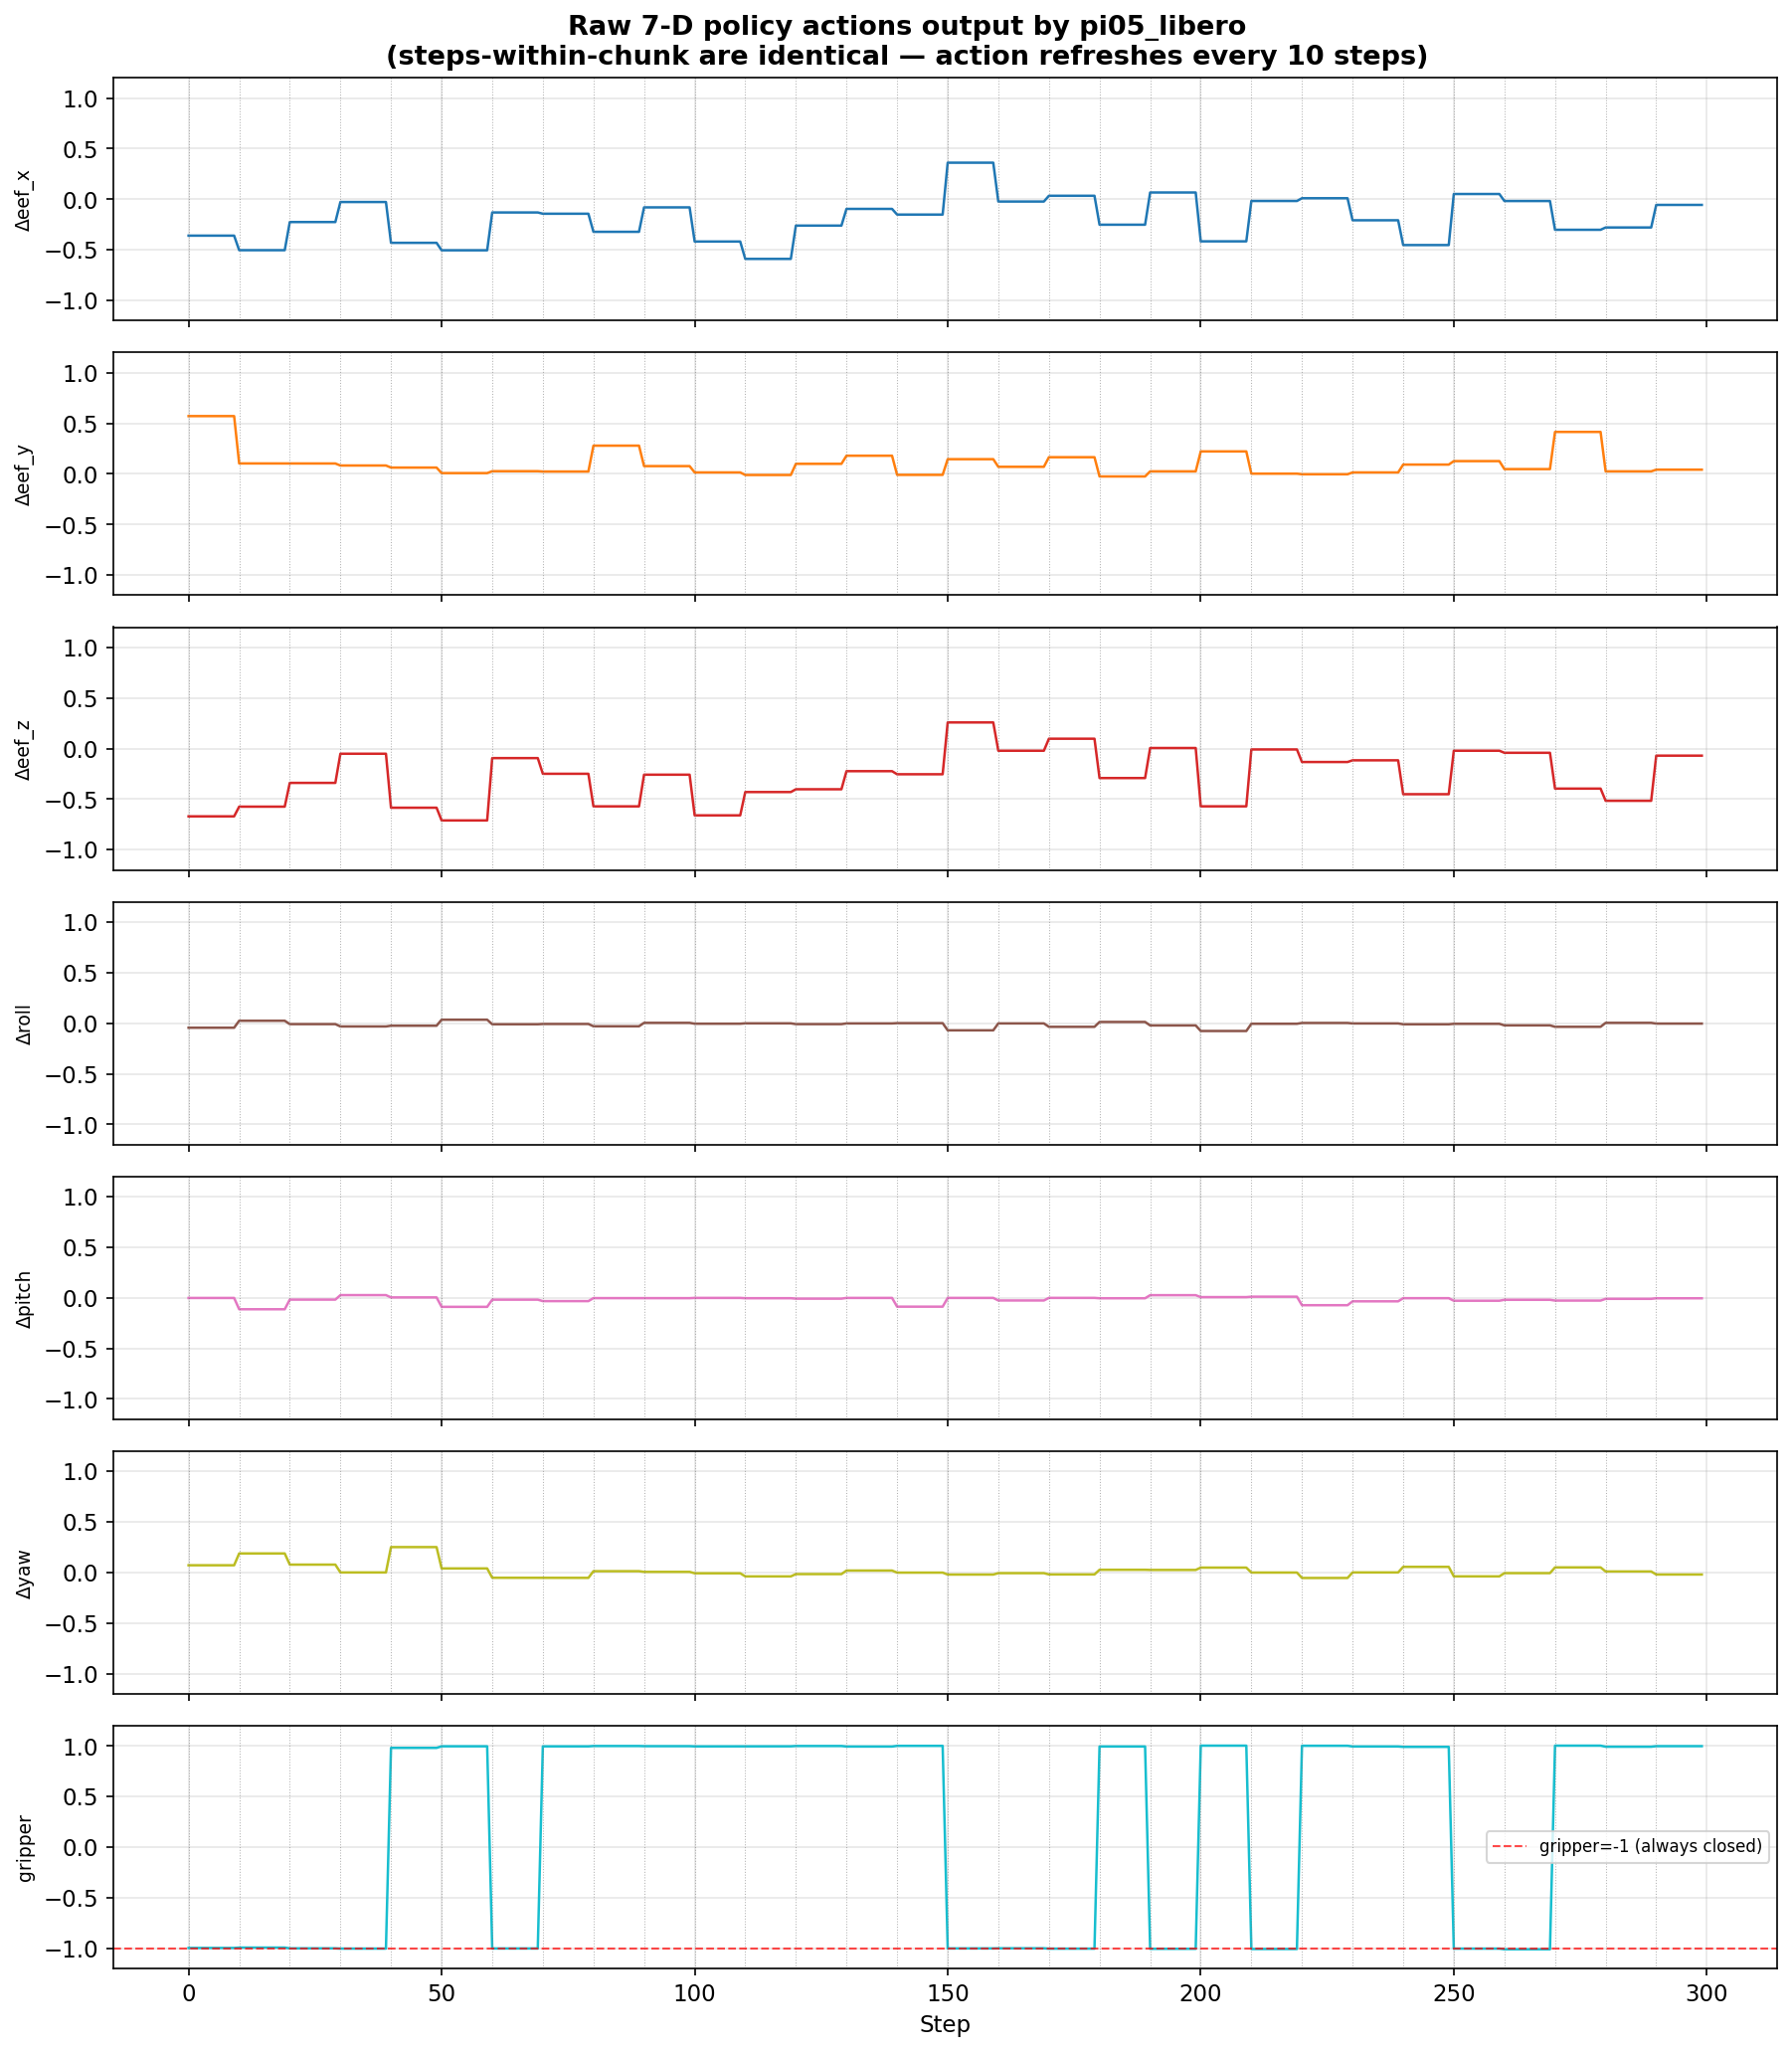
\includegraphics[width=\linewidth]{figures/late_stage_images/03_policy_actions_7d.png}
\caption{Raw 7-D end-effector action output by the zero-shot policy during the rollout: each action chunk is held constant for 10 steps before re-planning.}
\label{fig:zeroshot_actions}
\end{figure}

\begin{figure}[H]
\centering
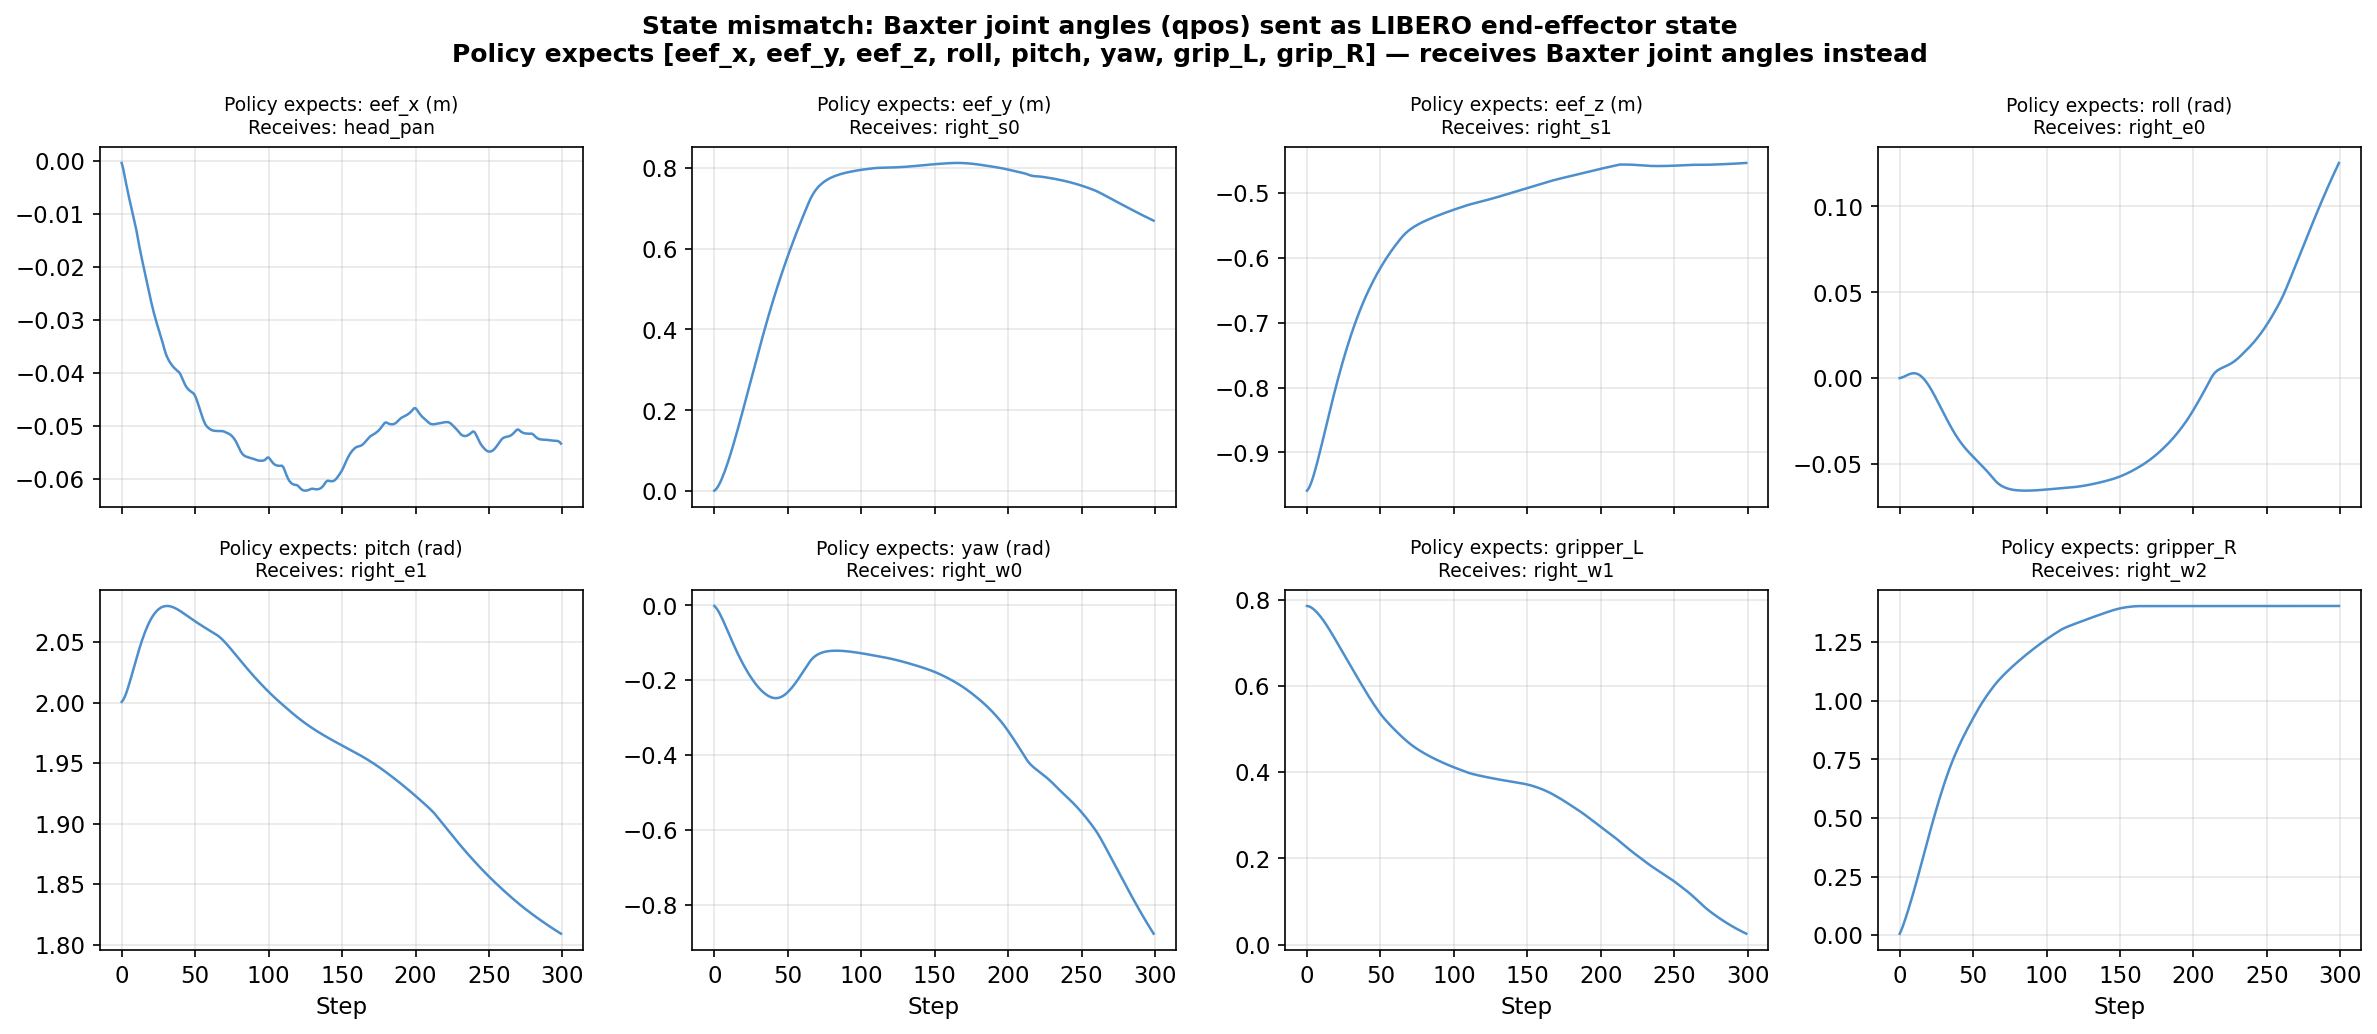
\includegraphics[width=\linewidth]{figures/late_stage_images/04_state_mismatch.png}
\caption{Zero-shot deployment diagnostic: each dimension of Baxter's raw joint-angle state (bottom labels) plotted against the semantically unrelated end-effector state dimension the pretrained policy interprets it as (top labels).}
\label{fig:zeroshot_diagnostics}
\end{figure}

\begin{figure}[H]
\centering
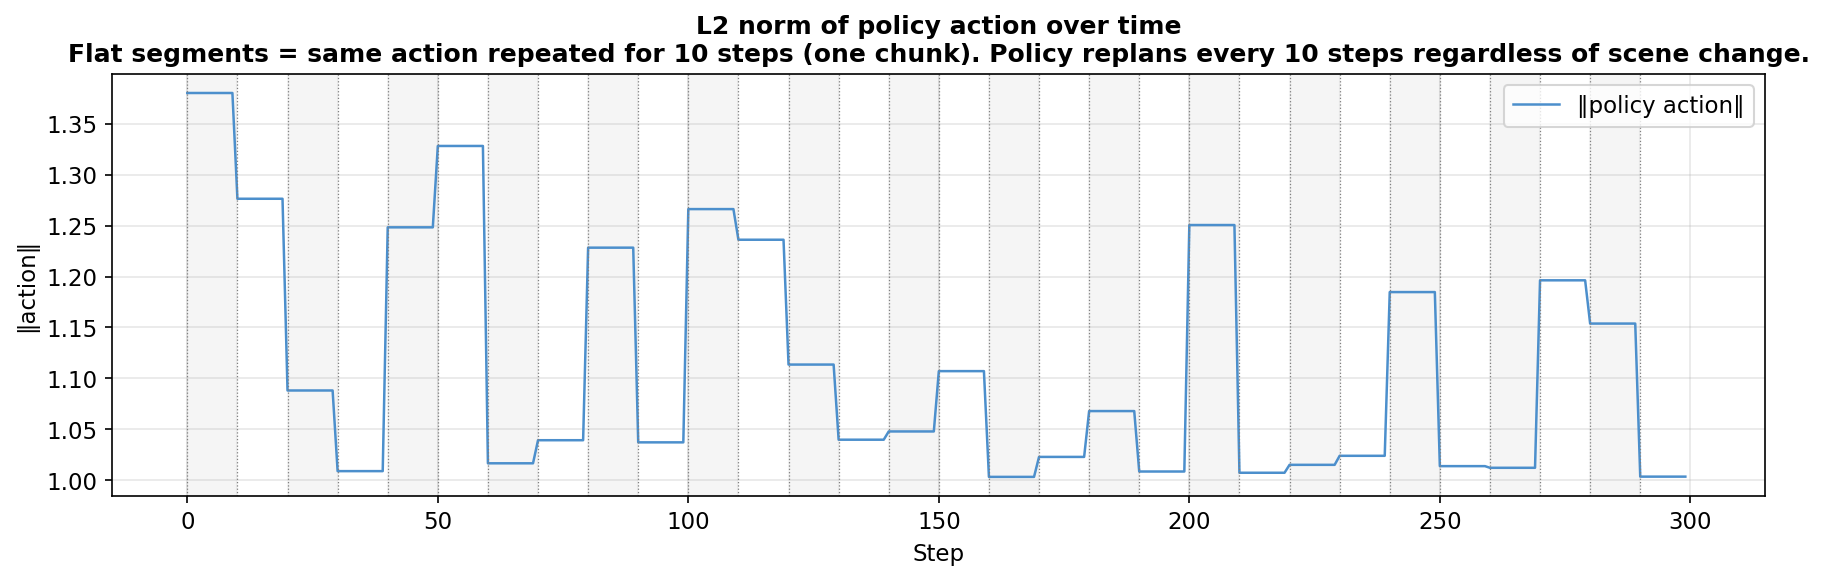
\includegraphics[width=\linewidth]{figures/late_stage_images/06_chunk_repetition.png}
\caption{L2 norm of the commanded action over the same rollout: the policy continues to re-plan large-magnitude actions every 10 steps regardless of scene state, rather than settling as the (non-existent, in this zero-shot case) task nears completion.}
\label{fig:zeroshot_l2norm}
\end{figure}

The Baxter platform and structured block-manipulation tasks introduced in Section~\ref{sec:demo-pipeline} differ substantially from the original $\pi$0.5 training data, making fine-tuning necessary. The objective is therefore to adapt the pretrained policy to the target robot and task using a relatively small demonstration dataset rather than training a policy from scratch.

\subsubsection{Parameter-Efficient Adaptation using LoRA}
Low-Rank Adaptation (LoRA) was used to fine-tune the pretrained $\pi$0.5 model. Instead of updating all 3 billion parameters, LoRA freezes the pretrained model and trains low-rank adapters within the attention layers.

Adapters were applied to both the 2B-parameter PaliGemma vision-language backbone and the 300M-parameter action expert. Using a rank of 16 resulted in approximately 30--50 million trainable parameters and reduced GPU memory usage to around 17\,GB, enabling training on a single RTX 5090 GPU.

LoRA enabled efficient evaluation of multiple datasets, action representations, and state configurations while preserving the pretrained model's visual and language capabilities, and the same adaptation strategy was reused without modification when extending the pipeline to the Franka and G1 embodiments in Section~\ref{sec:methodology-crossemb}.

\subsection{Development of the Demonstration Collection Pipeline}
\label{sec:demo-pipeline}

A demonstration collection pipeline was developed to generate task-specific data for fine-tuning the $\pi$0.5 model. Demonstrations were generated through scripted execution in MuJoCo, providing repeatable and scalable data collection. The pipeline consisted of four stages: task design, inverse kinematics trajectory generation, demonstration recording, and conversion to the LeRobot dataset format.

\subsubsection{Task Design}
The target task is to transform an initial block arrangement into a user-specified goal configuration. To simplify learning, the problem was decomposed into six reusable manipulation primitives involving three coloured blocks placed on a tabletop divided into near and far regions (Fig.~\ref{fig:workspace}):

\begin{itemize}[nosep]
\item Move the red block to the near side
\item Move the red block to the far side
\item Move the blue block to the near side
\item Move the blue block to the far side
\item Move the green block to the near side
\item Move the green block to the far side
\end{itemize}

These primitives can be combined by the VLM planner (Section~\ref{sec:vlm-planner}) to perform more complex rearrangement tasks (Table~\ref{tab:primitives}).

\begin{figure}[H]
\centering
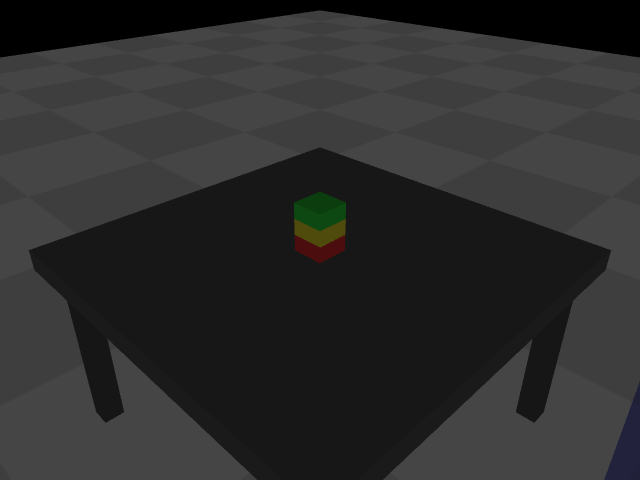
\includegraphics[width=0.85\linewidth]{figures/late_stage_images/mujoco_setup.png}
\caption{Tabletop workspace for execution of primitive tasks: blocks placed on a tabletop divided into near and far regions.}
\label{fig:workspace}
\end{figure}

\begin{table}[H]
\centering
\caption{Manipulation primitives used by the planner}
\label{tab:primitives}
\begin{tabular}{ll}
\toprule
\textbf{Object} & \textbf{Primitive Actions} \\
\midrule
Red & Move Near, Move Far \\
Blue & Move Near, Move Far \\
Green & Move Near, Move Far \\
\bottomrule
\end{tabular}
\end{table}

\subsubsection{Damped Least Squares Inverse Kinematics}
To generate demonstrations, a controller capable of reliably executing pick-and-place trajectories was required. For a desired end-effector displacement $\Delta x$, the corresponding joint update $\Delta q$ is computed as
\begin{equation}
\Delta q = J^T (J J^T + \lambda^2 I)^{-1} \Delta x
\label{eq:dls}
\end{equation}
where $J$ is the manipulator Jacobian and $\lambda$ is the damping coefficient. Damped Least Squares (DLS) inverse kinematics was selected for its numerical stability near singular configurations and its compatibility with simulation and the physical robot alike. This same controller design, unmodified in its mathematical form, was reused for the Franka and G1 demonstration-generation scripts in Section~\ref{sec:methodology-crossemb}, only the per-embodiment kinematic chain and reach margins differing.

\subsubsection{Scripted Demonstration Collection}
Demonstrations were generated autonomously through a scripted pick-and-place controller implemented within the MuJoCo simulation environment. Each episode followed a structured sequence: (1) move to a pre-grasp position above the target block; (2) descend towards the block; (3) close the gripper and establish grasp contact; (4) lift the object above the workspace; (5) transport the object to the target region; (6) lower the object and release the grasp; (7) return to a neutral configuration.

Scripted execution ensured consistent demonstrations and enabled rapid dataset generation without teleoperation. To improve generalisation, block positions were randomised at the start of each episode while maintaining task feasibility. A total of 600 demonstrations were collected for the Baxter dataset used in the checkpoints reported in Section~\ref{sec:results-sim}, with 100 demonstrations for each primitive task.

\subsubsection{Dataset Processing}
Recorded demonstrations were converted to the LeRobot dataset format required by the $\pi$0.5 training framework. Each sample contained workspace and wrist camera images, robot state information, a language instruction, and the corresponding action target. Dataset validation verified trajectory integrity and observation--action consistency before fine-tuning.

\subsection{Design of the Action Representation}
\label{sec:action-rep}

Two action representations were evaluated. Initial experiments used the velocity-control formulation of the original $\pi$0.5 framework, in which the policy predicts joint velocities. This was later replaced with position control, where the policy predicts target joint positions and a proportional controller generates the corresponding robot motions. The transition required new demonstrations with future joint configurations as action targets. Its impact on manipulation performance is evaluated in Section~\ref{sec:results-sim}.

The underlying reason velocity control proved difficult to learn reliably, established only after the fact through the train--inference mismatch analysis of Section~\ref{sec:results-sim}, is that a velocity target is a much noisier learning signal than a position target for a flow-matching policy operating on 10\,Hz-downsampled demonstrations: a velocity is a first-order difference of position, so any timing jitter or downsampling artefact in the demonstration data is amplified into the action label itself, whereas a position target remains well-defined regardless of the exact timing at which it is recorded. Position control effectively delegates timing-sensitive execution to the proportional controller (Section~\ref{sec:methodology}), leaving the learned policy responsible only for predicting a target configuration -- a strictly easier prediction problem -- which is consistent with the substantially higher block-lifted rates reported for every position-control checkpoint relative to the velocity-control baseline in Table~\ref{tab:lift_rate}. This same reasoning, rather than any embodiment-specific property of Baxter, is why position control was adopted unmodified as the default representation for the Franka and G1 extensions in Section~\ref{sec:methodology-crossemb}, without re-evaluating velocity control on either new embodiment.

\subsection{Fine-Tuning and Inference Pipeline}

\subsubsection{Training Configuration}
Each training sample consisted of workspace and wrist camera images, robot state information, and a language instruction. The model was trained to predict the corresponding action sequence using LoRA adapters, while the pretrained backbone remained frozen. Training used a batch size of 2, a cosine learning-rate schedule decaying from a peak of $2\times10^{-4}$ to a final value of $1\times10^{-5}$ (except \texttt{pos\_v3}'s warm-start continuation, which used a reduced peak of $5\times10^{-5}$ throughout, per Table~\ref{tab:training_metrics}), and the AdamW optimiser. Multiple training runs were performed to evaluate different action representations, datasets, and state configurations, with checkpoints saved every 10,000 training steps (Table~\ref{tab:finetuning_config}).

\begin{table}[H]
\centering
\caption{Fine-tuning configuration}
\label{tab:finetuning_config}
\begin{tabular}{ll}
\toprule
Model & $\pi$0.5 \\
Adaptation & LoRA \\
Framework & OpenPI \\
Dataset & LeRobot \\
Training Steps & Various (100k--500k) \\
Checkpoint Interval & 10k \\
Hardware & RTX 5090 (32\,GB) \\
\bottomrule
\end{tabular}
\end{table}

\subsubsection{Inference Architecture}
A two-process inference framework was developed, consisting of a GPU-based policy server and a simulation (or, for the real-robot deployment described in Section~\ref{sec:methodology-realrobot}, a ROS-driven robot) client communicating via WebSocket. At each timestep, the client sends camera observations, robot state information, and the task instruction to the policy server. The server applies the same preprocessing used during training, performs inference with the fine-tuned $\pi$0.5 model, and returns an action chunk for execution.

For position-control policies, predicted joint positions are executed by a proportional controller: $v = \mathrm{clip}(K_P (q_{\text{target}} - q), -v_{\max}, v_{\max})$, with $K_P = 40$ and $v_{\max} = 1.5$\,rad/s. This separates the \emph{where} (learned by the policy) from the \emph{how fast} (handled by the controller), substantially simplifying the learning problem. This inference framework provides a consistent environment for checkpoint evaluation and policy comparison, and is reused, with the modifications described in Section~\ref{sec:methodology-realrobot}, for the physical robot.

\subsection{Vision-Language Planner}
\label{sec:vlm-planner}

A Vision--Language Model (VLM) was introduced to provide high-level task planning within the proposed human-robot collaboration framework. While the fine-tuned $\pi$0.5 policy executes individual manipulation primitives, it has no knowledge of the desired final scene configuration. The VLM planner addresses this limitation by converting a goal scene into an ordered sequence of manipulation primitives (Fig.~\ref{fig:vlm_pipeline}). This section describes the planner in substantially more detail than the late-stage report, reflecting the fact that its design, prompting strategy, and closed-loop integration with the policy were completed during this final stage.

\begin{figure}[H]
\centering
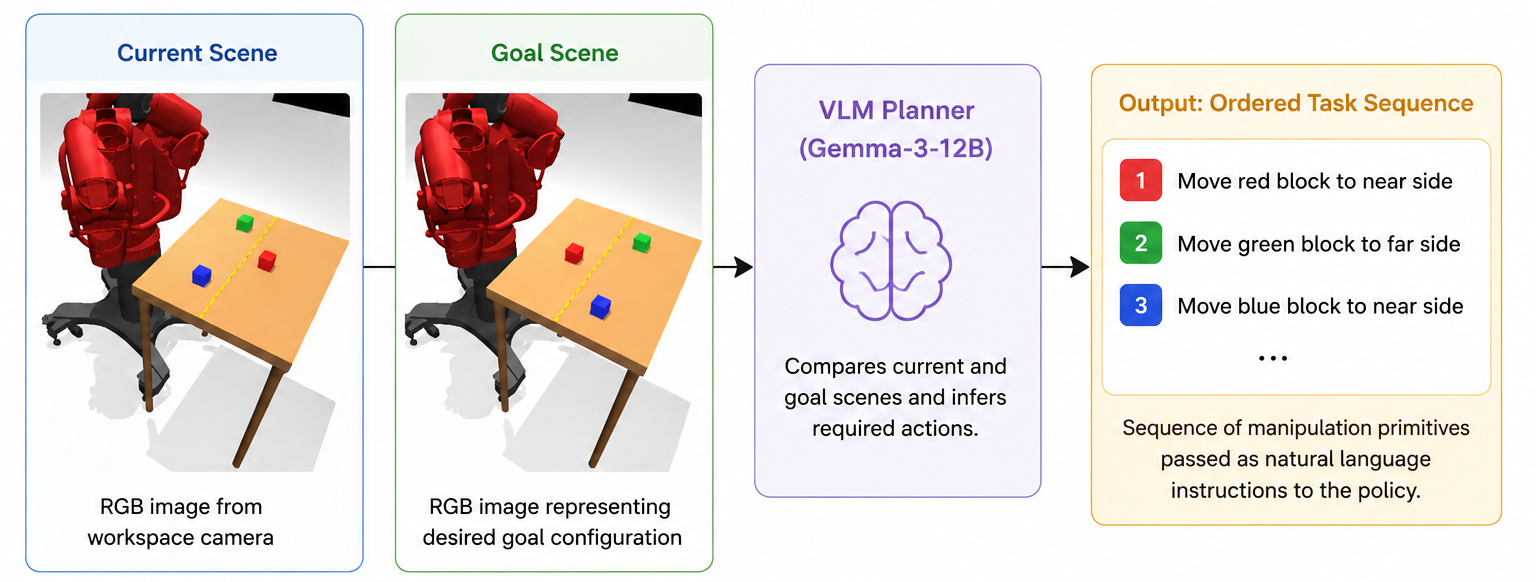
\includegraphics[width=0.85\linewidth]{figures/late_stage_images/VLM_planner.png}
\caption{High-level VLM planning pipeline: the current and goal workspace images are compared to infer the required sequence of manipulation primitives.}
\label{fig:vlm_pipeline}
\end{figure}

\subsubsection{Planner Implementation}
Gemma-3-12B (\texttt{google/gemma-3-12b-it}) was selected as the planning model due to its multimodal reasoning capability and its ability to jointly process two images and text in a single query. The planner receives the current workspace image together with a goal-state image and identifies the differences between the two scenes.

\subsubsection{Per-Block Independent Querying}
A key design decision, motivated directly by the early-stage monitoring pilot (Section~\ref{sec:early-monitoring}), is to query the VLM once per block colour rather than asking it to reason about all three blocks simultaneously. That pilot found that Gemma-3-12B produced accurate free-form natural-language scene descriptions but unreliable, inconsistent structured output when asked to report the state of multiple objects at once -- a well-documented weakness of VLMs when required to bind attributes (colour, position) to multiple instances of similar objects in a single response. The planner sidesteps this weakness entirely by construction: for each of the three block colours in turn, it is shown the same current/goal image pair and asked a single, tightly scoped question restricted to that colour alone,
\begin{quote}
\small\ttfamily
Focus ONLY on the \{color\} block. Ignore all other blocks. \\
Answer in EXACTLY this format (two lines, no extra text): \\
current: near \\
goal: far
\end{quote}
with the workspace's near/far dividing line explained in the same prompt relative to the robot arm and the image frame. The two-line, fixed-vocabulary answer format is deliberately far more constrained than the free-form descriptions used during the early-stage evaluation, and is parsed with a strict, line-anchored parser that only accepts the literal tokens \texttt{near} or \texttt{far}; if a response fails to parse for a given block, that block is skipped with a warning rather than silently misinterpreted. If the parsed current and goal positions differ for a colour, the corresponding primitive (\emph{``move the \{color\} block to the \{goal\} side''}) is appended to the task list; if they agree, no primitive is issued for that block. This directly implements the intended behaviour of Table~\ref{tab:primitives} while making the planner's structured-output failure mode -- identified as a key early-stage insight -- explicit and recoverable rather than silent.

\subsubsection{Closed-Loop Goal Checking and Re-Planning}
A second, independent query asks the VLM a single yes/no question -- whether all three blocks are on the same side of the dividing line in both the current and goal images -- used as a goal-satisfaction check that is decoupled from the per-block planning query. This check is used both before planning begins (to short-circuit planning entirely if the goal is already satisfied) and after each executed primitive, so that the system can detect early goal completion without executing the full planned sequence. If, after all currently planned primitives have been executed, the goal check still returns \emph{no}, the planner re-renders the scene and repeats the plan--execute--check cycle, up to a configurable maximum number of rounds (three, in the current implementation). This closed-loop behaviour is precisely the ``dynamic re-planning'' capability that the late-stage report identified as a future-work item for evaluating human intervention in the workspace: the mechanism required for it -- re-observe, re-plan, re-check -- is now implemented and exercised automatically after every primitive, and is the mechanism that will be triggered by a human deliberately altering the scene mid-task in the collective-task evaluation of Section~\ref{sec:methodology-hrc}.

The round limit of three was chosen as a pragmatic bound rather than derived from any theoretical argument: since each round involves at least one VLM forward pass (three per-block queries plus one goal check) and one full policy-execution primitive that itself takes up to \texttt{MAX\_STEPS} $= 600$ control steps (60\,s at 10\,Hz) to complete, an unbounded retry loop risks a single pathological configuration (for example, a persistent planner misclassification) consuming an unreasonable amount of session time; three rounds was judged, on the basis of the qualitative development trials in Section~\ref{sec:results-vlm}, to be enough for the closed-loop mechanism to recover from an isolated misclassification or an intervening human action without allowing a genuinely stuck configuration to run indefinitely, though this bound has not itself been tuned against the quantitative planner-accuracy data that Section~\ref{sec:results-vlm} identifies as still pending.

\subsubsection{Goal Space and Integration with the Policy}
The full goal space spans all $2^3 = 8$ near/far combinations across the three blocks, with a goal image pre-rendered for each combination (Fig.~\ref{fig:goal_grid}). At runtime, each planned primitive is passed as a natural-language instruction to the fine-tuned $\pi$0.5 policy exactly as in the single-task evaluation of Section~\ref{sec:results-sim}, and is executed to completion (or a per-task step budget) using the same 10\,Hz closed-loop websocket inference and P-controller execution described above, including the grasp-latch and hysteresis logic of Section~\ref{sec:results-sim} that prevents premature gripper release during transport. This hierarchical decomposition enables the system to perform object arrangements that were never explicitly demonstrated during fine-tuning, since only the six single-block primitives, not their compositions, appear in the training data.

\begin{figure}[H]
\centering
\begin{subfigure}[b]{0.22\linewidth}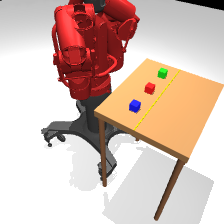
\includegraphics[width=\linewidth]{figures/goal_images_6task/red_near_blue_near_green_near.png}\caption*{all near}\end{subfigure}
\begin{subfigure}[b]{0.22\linewidth}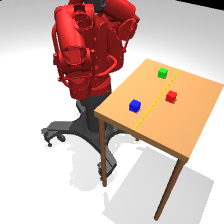
\includegraphics[width=\linewidth]{figures/goal_images_6task/red_far_blue_near_green_near.png}\caption*{R far}\end{subfigure}
\begin{subfigure}[b]{0.22\linewidth}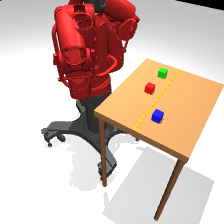
\includegraphics[width=\linewidth]{figures/goal_images_6task/red_near_blue_far_green_near.png}\caption*{B far}\end{subfigure}
\begin{subfigure}[b]{0.22\linewidth}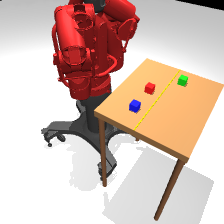
\includegraphics[width=\linewidth]{figures/goal_images_6task/red_near_blue_near_green_far.png}\caption*{G far}\end{subfigure}

\begin{subfigure}[b]{0.22\linewidth}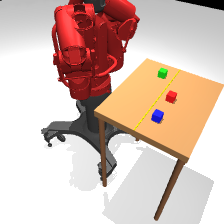
\includegraphics[width=\linewidth]{figures/goal_images_6task/red_far_blue_far_green_near.png}\caption*{R,B far}\end{subfigure}
\begin{subfigure}[b]{0.22\linewidth}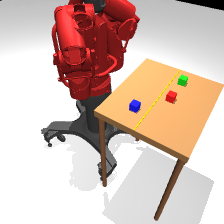
\includegraphics[width=\linewidth]{figures/goal_images_6task/red_far_blue_near_green_far.png}\caption*{R,G far}\end{subfigure}
\begin{subfigure}[b]{0.22\linewidth}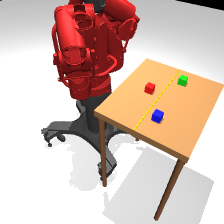
\includegraphics[width=\linewidth]{figures/goal_images_6task/red_near_blue_far_green_far.png}\caption*{B,G far}\end{subfigure}
\begin{subfigure}[b]{0.22\linewidth}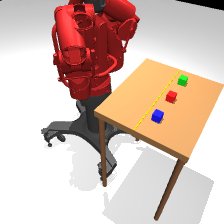
\includegraphics[width=\linewidth]{figures/goal_images_6task/red_far_blue_far_green_far.png}\caption*{all far}\end{subfigure}
\caption{The full $2^3=8$-configuration goal space (red/blue/green $\times$ near/far) used by the VLM planner; each image is pre-rendered and supplied as the goal observation for the corresponding configuration.}
\label{fig:goal_grid}
\end{figure}

\subsection{Cross-Embodiment Generalisability}
\label{sec:methodology-crossemb}

The first new experimental thread extends the fine-tuning and demonstration-collection pipeline described above from Baxter alone to two additional embodiments, Franka Emika Panda and Unitree G1 (single arm), with the eventual aim of training a \emph{single} cross-embodiment $\pi$0.5 policy jointly on all three, rather than three independent solo policies. This is a direct empirical test of RQ4: whether $\pi$0.5's pretraining-time claim of open-world, cross-embodiment generalisation extends to the fine-tuning regime used throughout this project.

\begin{figure}[H]
\centering
\begin{subfigure}[b]{0.32\linewidth}
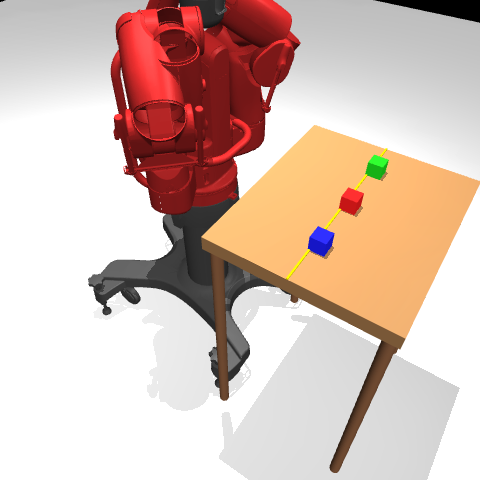
\includegraphics[width=\linewidth]{figures/generated/baxter_twoblocks.png}
\caption{Baxter}
\end{subfigure}
\hfill
\begin{subfigure}[b]{0.32\linewidth}
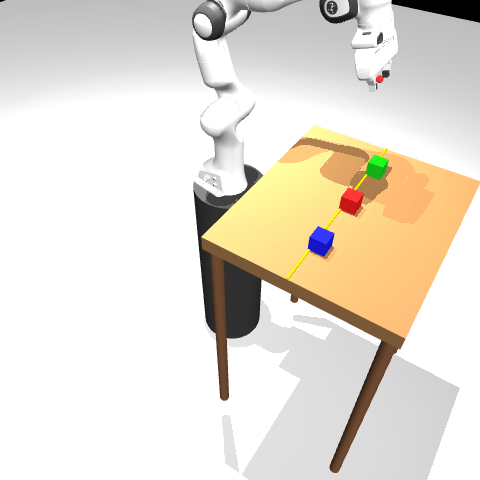
\includegraphics[width=\linewidth]{figures/generated/franka_twoblocks.png}
\caption{Franka Emika Panda}
\end{subfigure}
\hfill
\begin{subfigure}[b]{0.32\linewidth}
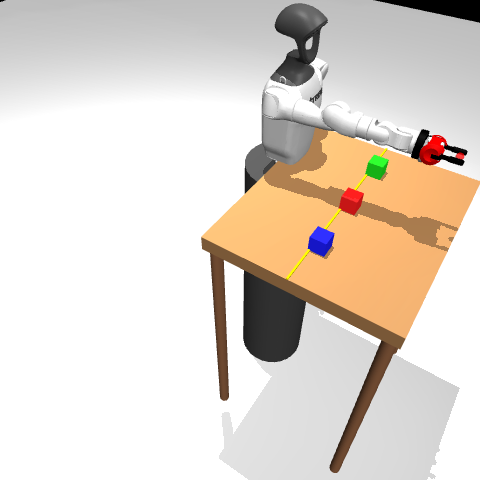
\includegraphics[width=\linewidth]{figures/generated/g1_twoblocks.png}
\caption{Unitree G1 (right arm)}
\end{subfigure}
\caption{The three-block tabletop environment reconstructed for each of the three embodiments, sharing an identical table, dividing line, and block layout so that demonstrations and evaluation criteria remain directly comparable across robots.}
\label{fig:cross_embodiment_scenes}
\end{figure}

\subsubsection{Scope Decisions}
Several scope decisions were made to keep the extension tractable within the project timeline while preserving comparability with the existing Baxter pipeline. Development was conducted entirely in simulation (no physical Franka or G1 hardware). G1's lower body was locked (no legs, no free-floating base, no waist joints, fixed pedestal mount) and only the right arm was used, mirroring the convention already used for Baxter, whose demonstrations likewise drive only the right arm despite the robot being physically dual-armed. Both Franka and G1 were fitted with a simplified 1-DOF parallel gripper: Franka's native tendon-coupled parallel gripper was used directly, while G1's native multi-fingered Dex3 hand was replaced with a copy of Baxter's own Rethink parallel-jaw gripper subtree, reused verbatim for design and dataset consistency across all three embodiments (Fig.~\ref{fig:cross_embodiment_scenes}). The full six-primitive task set from Table~\ref{tab:primitives} was targeted on both new robots, with the final achieved task coverage differing by embodiment (Section~\ref{sec:results-crossemb}) due to embodiment-specific reach and collision constraints rather than a deliberate reduction in scope.

\subsubsection{Scene and Demonstration Pipeline}
New MuJoCo scenes (\texttt{franka\_twoblocks.xml}, \texttt{g1\_twoblocks.xml}) were constructed reusing the same table, dividing line, and three-block layout as the Baxter environment, with each robot's own manufacturer mesh assets and kinematic chain. Demonstration generation follows exactly the same four-stage pipeline as Section~\ref{sec:demo-pipeline} -- task design, DLS inverse-kinematics trajectory generation (Eq.~\ref{eq:dls}, unmodified in form), scripted recording, and LeRobot conversion -- via new per-embodiment scripts (\texttt{record\_demos\_franka\_pos.py}, \texttt{record\_demos\_g1\_pos.py}, \texttt{convert\_to\_lerobot\_franka.py}, \texttt{convert\_to\_lerobot\_g1.py}) that mirror the structure of the existing Baxter scripts. The resulting per-embodiment datasets share an identical schema to the Baxter dataset: $(224,224,3)$ uint8 workspace and wrist images, an 11-dimensional state vector (7 joint angles, gripper norm, 3D end-effector position), and an 8-dimensional action vector (7 joint targets, gripper norm), so that the three datasets can be mixed during joint training without further reconciliation.

Because the scripted DLS controller is not perfectly reliable for every embodiment and task combination (a property already true of, and accounted for, in the existing Baxter dataset), demonstrations were deliberately over-recorded relative to the target dataset size and filtered to successful episodes only, rather than treating anything below 100\% scripted success as unusable.

\subsubsection{Reach-Margin Methodology}
A recurring failure mode during scene construction was a task/embodiment combination sitting right at the edge of a robot's reachable workspace, producing inverse-kinematics instability or collapsed grasp behaviour that superficially resembled a task-specific bug but was in fact a geometric reach-margin problem. A repeatable diagnostic procedure was developed and applied across both new embodiments: for a candidate base position and task, a batch of scripted episodes is run and the yield (fraction reaching a successful grasp and placement) is recorded before committing to full-scale demonstration collection; where yield is low, the robot's base position or the target region is adjusted and the batch is re-run, rather than assuming the task is infeasible from a single failed trial. This pattern, first identified while diagnosing G1's shorter-arm trade-off between its base position and both near- and far-side reach, is recorded as a reusable methodology for any future embodiment extension of this pipeline.

\subsubsection{Representative Engineering Issues}
\label{sec:crossemb-bugs}

The reach-margin methodology of the previous section was one recurring pattern among a larger set of embodiment-specific issues encountered and resolved during scene construction, several of which are recorded here as they illustrate a broader point returned to in Section~\ref{sec:discussion}: that most cross-embodiment problems were traceable to a specific, identifiable cause rather than being vague ``embodiment differences''.

G1's wrist camera initially rendered as a dark, extreme close-up (mean pixel intensity $\approx 20$, versus $\approx 215$ for the scene camera), traced to the camera being attached with Baxter's numeric mounting offset relative to the wrong parent frame -- G1's wrist-to-gripper rotation differs from Baxter's, so a Baxter-derived offset placed the camera facing into the gripper's own body. Re-attaching the camera to the correct parent frame, with an offset translated to account for G1's copied gripper subtree, restored an expected close, gripper-dominated wrist view (mean pixel $\approx 57$--64, visually consistent with Baxter's own wrist camera).

G1 also initially achieved 0\% success on all six tasks due to self-collision: MuJoCo's default collision bitmask meant the arm's gripper-base collision geometry persistently contacted the torso/pedestal partway through a joint-space sweep, a distinction Baxter's own model avoids through hand-tuned collision bitmasks that Baxter's dual-arm geometry required but G1's fixed-pedestal, single-arm configuration did not. Disabling self-collision on G1's locked torso and pedestal, while leaving the gripper's own dedicated contact classes untouched, resolved this without affecting genuine object/table contact. A related issue was G1's home pose placing the gripper very low near the pedestal, so that a large joint-space interpolation from home to a pre-grasp pose could swing intermediate arm links through table height; raising the home keyframe to an elevated pose resolved this and, as a side effect, reduced the joint-space distance to every pre-grasp pose, independently lowering collision risk.

For Franka, the first end-to-end test likewise achieved 0\% success, traced to the six-dimensional descent phase's target orientation being derived via forward kinematics from an unconstrained, randomly-searched pre-grasp joint configuration -- since that configuration was found without any orientation objective, the resulting ``target'' orientation was not a physically sensible grasp pose, and the combined position-and-orientation inverse-kinematics objective diverged rather than converged. Replacing this with a fixed canonical target orientation (gripper pointing straight down, defined independently of any particular joint configuration), and re-searching the pre-grasp configuration to be consistent with that fixed target, resolved red and blue block tasks; green-block tasks required a further fix once diagnosis showed the pre-grasp configuration sitting within 0.03\,rad of a joint limit, producing a poorly-conditioned Jacobian during descent -- adding a joint-limit-proximity penalty to the pre-grasp search resolved this.

A further category of issues concerned grasp retention rather than reaching: blocks slipping out of the gripper during long carry-phase dwells (traced to a stale, over-generous timeout inherited from Baxter's script combined with too-abrupt gripper closure), Franka's stock parallel-gripper actuator being mechanically too weak to hold a stiffened grip without renewed slippage, and blocks sliding several centimetres upon gripper release because the place phase converged with the block still fractionally above the table rather than in firm contact. Each was resolved individually (a shortened, tighter carry-phase timeout with a ramped rather than instantaneous gripper closure; a stiffened gripper actuator gain; and a short settle hold before release) rather than by a single generic ``increase robustness'' change, consistent with the project's broader preference, established in the late stage, for diagnosing a specific mechanism before applying a fix.

\subsubsection{Joint Multi-Embodiment Training}
To support training a single policy across all three embodiments' datasets without merging them into one physically combined dataset, new mixture-loading support was added to the OpenPI training configuration, rather than concatenating the three LeRobot datasets at conversion time. Physically merging the datasets was rejected because a single merged dataset would receive a single set of normalisation statistics computed jointly across all three embodiments' state and action values, despite Baxter's, Franka's, and G1's joint angles occupying different physical ranges; instead, each embodiment's dataset retains its own normalisation statistics, and the three are combined at data-loading time through a weighted mixture (an equal $1.0/1.0/1.0$ weighting as an unoptimised starting default). This design allows a fair, direct comparison between the joint cross-embodiment policy and three independently fine-tuned solo policies (one per embodiment, including reuse of the existing, already-validated Baxter \texttt{pos\_v3} run as the Baxter solo baseline), which is the comparison this experiment is ultimately designed to produce.

\subsection{Human-Robot Collaborative Task}
\label{sec:methodology-hrc}

The second new experimental thread defines and readies for evaluation the \emph{collective task}: the end-to-end evaluation of the complete planner--policy framework on a genuinely collaborative rearrangement task, directly answering RQ5 and completing the human-robot collaboration evaluation outlined as future work in the late-stage report. Fig.~\ref{fig:hrc_concept} shows the early conceptual sketch of subtask allocation between robot and human that first motivated this direction.

\begin{figure}[H]
\centering
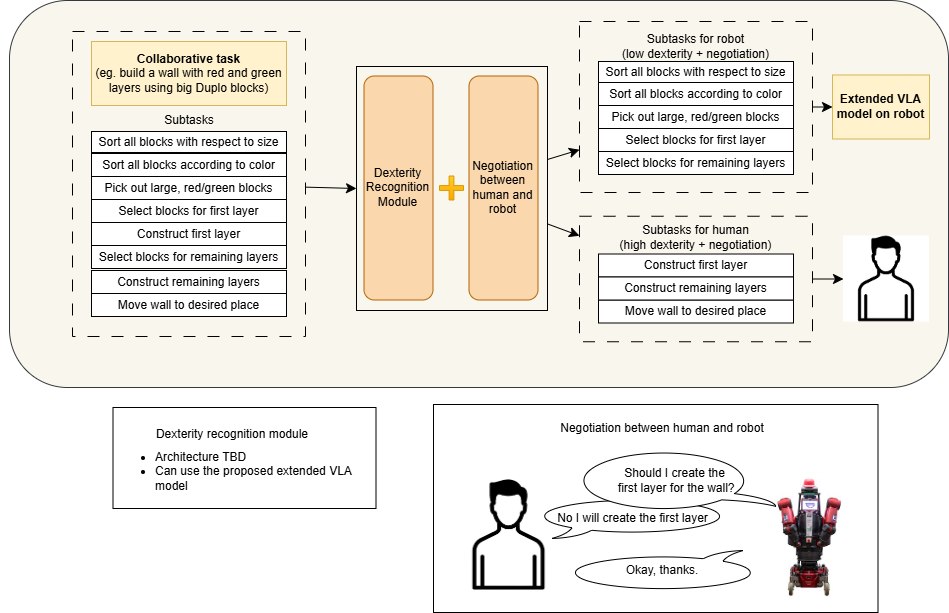
\includegraphics[width=0.85\linewidth]{figures/late_stage_images/hrc.drawio.png}
\caption{Early conceptual sketch of the collaborative task allocation problem: subtasks are split between robot and human by dexterity requirement, with a negotiation step reconciling who performs which subtask. This early concept motivates the collective-task protocol defined below, though the implemented protocol allocates subtasks by planner-detected configuration difference rather than a separate dexterity-recognition module.}
\label{fig:hrc_concept}
\end{figure}

\subsubsection{Task Definition}
Given an initial and goal workspace configuration, the Vision--Language planner (Section~\ref{sec:vlm-planner}) generates a sequence of manipulation primitives, which are executed by the fine-tuned $\pi$0.5 policy exactly as in the single-planner evaluation of Section~\ref{sec:results-vlm}. What distinguishes the \emph{collective} task from this planner--policy evaluation alone is that a human partner shares the workspace and may act on it at two points: (i) before execution begins, by placing the blocks in an arbitrary initial configuration not otherwise generated by the system, and (ii) mid-execution, by manually repositioning one or more blocks between planned primitives, exercising the closed-loop goal-check--replan cycle of Section~\ref{sec:vlm-planner} under a genuine, rather than simulated, source of scene change. Because the planner re-renders the scene and re-checks the goal after every executed primitive rather than only at the start, a human intervention occurring at any point in the sequence is expected to be picked up at the next check and folded into a revised plan, without requiring a separate ``interruption'' code path.

This design choice -- detecting intervention implicitly through scene re-observation, rather than through an explicit signal from the human (a button press, a spoken command, or a dedicated ``I've changed something'' message) -- is a deliberate simplification with a specific cost. It means the system cannot distinguish a human intervention from its own execution imperfectly finishing a primitive (for example, a block ending up a few centimetres short of its intended near/far region), since both present identically as ``the scene does not match what the planner expected after this primitive''. This is an acceptable simplification for the near/far task granularity used throughout this project, where the two situations are unlikely to be confused in practice, but it does mean the replanning-trigger and replanning-correctness metrics defined below cannot, on their own, separate ``the system correctly detected a human's action'' from ``the system correctly detected its own execution error and is recovering from it'' -- both are folded into the same re-planning mechanism by construction, and distinguishing them, if required, would need to be logged separately at trial time by the human running the session rather than inferred from the system's own behaviour.

\subsubsection{Evaluation Protocol and Metric}
Performance is measured using a collaborative task success metric, defined at three increasingly strict levels, mirroring the three-level evaluation methodology already used for the single-policy results in Section~\ref{sec:results-sim}: \emph{primitive skill success} (did the specified block reach the correct side, regardless of manipulation quality), \emph{manipulation success} (was the full approach--grasp--lift--transport--release sequence completed cleanly), and \emph{collaborative task success} (did the complete planner--policy system, across every primitive in the plan, transform the initial configuration -- as left by the human -- into the specified goal configuration). A trial is considered a successful collaborative task only if collaborative task success is achieved without manual correction of the robot's actions, though human modification of the block configuration between primitives is treated as an expected part of the task rather than a failure condition. A secondary metric records, for trials that include a mid-execution human intervention, whether the system's re-plan after the intervention was both triggered (via the goal check returning \emph{no} when it otherwise would have returned \emph{yes}) and correct (matching the primitives an independent oracle would generate for the new configuration), to separate replanning-trigger reliability from re-planning correctness.

This protocol is fully specified and the supporting closed-loop mechanism is implemented (Section~\ref{sec:vlm-planner}); the trials themselves, across a range of initial/goal configuration pairs and intervention timings, are the immediate next step of the project and are reported as pending in Section~\ref{sec:results-hrc}.

\subsection{Real-Robot Deployment}
\label{sec:methodology-realrobot}

The third new experimental thread moves the validated simulation pipeline onto a physical Baxter robot, addressing RQ6.

\subsubsection{Deployment Architecture}
The physical deployment splits computation across two machines, reflecting the physical location of the available sensors and compute. A remote control laptop runs ROS Indigo and the \texttt{baxter\_interface} Python 2.7 client library, with direct access to the robot's joint state, gripper state, and its built-in wrist (right-hand) camera over Baxter's native ROS topics; this laptop has no GPU suitable for policy inference. The GPU used for policy inference is a separate, stationary lab PC, which also has an Intel RealSense camera attached directly to it, providing the workspace/scene view. Rather than routing the scene camera's video stream through the control laptop -- which is not physically connected to it and would add an unnecessary network hop -- the scene image is captured locally on the lab PC and injected directly into the observation dictionary by a wrapper (\texttt{serve\_policy\_realsense.py}) around the OpenPI websocket policy server, immediately before each inference call. The remote laptop's client (\texttt{baxter\_policy\_client.py}) therefore sends only the wrist-camera image, the 11-dimensional robot state, and the language prompt over the websocket; the wire format expected by the policy server is otherwise unchanged from the simulation client used throughout Sections~\ref{sec:demo-pipeline}--\ref{sec:vlm-planner}, so the fine-tuned policy itself required no modification for physical deployment.

This two-machine split was chosen over the alternative of running everything on the control laptop (piping its ROS topics to a remote GPU only for the neural network forward pass) because the laptop's ROS Indigo installation is tied to Python 2.7, which cannot run the modern Python 3 dependencies (JAX, PyTorch, and the OpenPI training stack) that $\pi$0.5 inference requires; splitting the system along this existing Python 2/3 boundary, rather than attempting to bridge it within a single process, follows the same modular, independently-swappable-components philosophy adopted for the planner--policy split described in Section~\ref{sec:design-approach}. The websocket protocol used for this split is identical to the one already used between the simulation client and the policy server (Section~\ref{sec:methodology}), which is what allows the real-robot client to be a comparatively small, self-contained script rather than a rewrite of the inference stack: the policy server has no way to distinguish a simulation client from a real-robot client, since both send the same observation schema. The only latency-relevant consequence of the split is the added network round-trip between the two machines, which sits within the same roughly 100\,ms inference gap between action chunks that the simulation architecture was already designed to tolerate (Section~\ref{sec:methodology}'s velocity command timeout of 1.0\,s was chosen with exactly this gap in mind), so no additional real-time budgeting was required specifically for the physical deployment.

\subsubsection{Control and Safety}
The real-robot client reuses the same P-controller and 10\,Hz replanning cadence as the simulation inference architecture (Section~\ref{sec:methodology}), converting each predicted joint-position target into a velocity command clipped to $\pm 1.5$\,rad/s, and executes the same grasp-latch and release-hysteresis logic used in simulation (Section~\ref{sec:results-sim}) to prevent the policy's occasional close--open--close prediction artefacts from dropping a grasped object during transport. Two safety measures specific to physical deployment were added: the arm's velocity command timeout was extended from the ROS default of 0.2\,s to 1.0\,s, since the roughly 100\,ms round-trip inference gap between action chunks would otherwise cause the low-level controller to fall back into position-hold mode between every chunk; and the client installs a SIGINT handler that immediately commands zero joint velocities and exits velocity-control mode before the process terminates, so that an operator's Ctrl-C reliably stops the arm rather than leaving a stale velocity command in effect.

\subsubsection{Validation Protocol}
The first physical validation milestone is single-block pick-and-place: executing task~0 (move the red block to the far side) -- the best-performing task for the strongest simulation checkpoint, \texttt{pos\_v3}, in Table~\ref{tab:trial_success} -- on the physical robot, under the same trial-level success criterion used in simulation (the block crossing the workspace divider). This isolates the sim-to-real question from the compounded, multi-task, planner-driven evaluation of Sections~\ref{sec:methodology-crossemb} and~\ref{sec:methodology-hrc}, and is intended as the first of a set of trials extending to the full six-primitive set once single-block execution is validated. At the time of writing, the deployment architecture above is implemented and the client/server pair has not yet been exercised on the physical robot; results are reported as pending in Section~\ref{sec:results-realrobot}.

\subsection{Evaluation Methodology}

The overarching objective of this research is a hierarchical human-robot collaboration system capable of transforming an initial workspace into a user-specified goal configuration, on a robot that is not restricted to a single embodiment, and while remaining responsive to a human partner. A single end-to-end pass/fail metric would not, on its own, distinguish a system that fails because the VLM planner misreads the scene from one that fails because the policy misses a grasp, from one that fails because a fine-tuned policy does not transfer to a second embodiment -- three qualitatively different problems requiring three different fixes. Since this capability depends on multiple intermediate components, evaluation is instead performed at several levels, extending the three-level methodology used in the late-stage report with three further levels corresponding to the new experimental threads above, so that a failure at any level of this final stage's evaluation can be attributed to the specific component responsible for it.

\begin{enumerate}[nosep]
\item \textbf{Primitive skill success} -- whether the policy performs the requested single-block task, measured without regard to manipulation quality (Section~\ref{sec:results-sim}).
\item \textbf{Manipulation success} -- whether the full pick-and-place sequence (approach, grasp, lift, transport, release) is completed cleanly, excluding accidental success from pushing (Section~\ref{sec:results-sim}).
\item \textbf{VLM planner accuracy} -- whether the planner correctly identifies, per block, whether it needs to move and in which direction, evaluated independently of policy execution by comparing planner output against the ground-truth configuration difference (Section~\ref{sec:results-vlm}).
\item \textbf{Cross-embodiment task success and transfer} -- per-embodiment primitive and manipulation success for the jointly trained policy, compared against the corresponding independently fine-tuned solo policy for the same embodiment, to quantify positive or negative skill transfer (Section~\ref{sec:results-crossemb}).
\item \textbf{Collaborative task success} -- whether the complete planner--policy system transforms a human-specified initial configuration into a human-specified goal configuration, including correct re-planning after a mid-execution human intervention (Section~\ref{sec:results-hrc}).
\item \textbf{Sim-to-real transfer} -- trial-level success of the fine-tuned policy on the physical Baxter robot, compared directly against the matching simulation checkpoint's success rate on the same task, to quantify the sim-to-real gap (Section~\ref{sec:results-realrobot}).
\end{enumerate}

% =====================================================================
\section{Results}
\label{sec:results}

\subsection{Simulation Policy Evaluation}
\label{sec:results-sim}

This section reports the mature, completed evaluation of the Baxter manipulation policy across five checkpoints, first presented in the late-stage report and reproduced here as the empirical foundation the newer experiments build on.

\subsubsection{Velocity-Control Policy Evaluation}

Initial fine-tuning experiments employed a velocity-control action representation in which the policy predicted joint velocity commands. The policy demonstrated clear language grounding by consistently approaching the correct coloured block, indicating that it had learned the relationship between visual observations, language instructions, and task objectives.

However, reliable manipulation was not achieved. The \texttt{vel\_100k} checkpoint achieved a 0\% success rate across 40 evaluation trials and failed to lift the block in any trial (Table~\ref{tab:trial_success}). Mean gripper close steps of 762 and 940 for the red-far and red-near tasks indicate that the gripper remained open throughout most of the episode, causing the robot to push the block rather than grasp it.

These results suggested that the policy had learned \emph{what} task to perform but not \emph{how} to execute it, motivating further investigation into train--inference mismatches and the subsequent transition to position-control actions.

\subsubsection{Analysis of Train--Inference Mismatches}

A significant part of the project involved identifying train--inference mismatches that limited policy performance. Four major issues were identified and resolved.

The first involved incorrect action targets during dataset generation. Actions were initially recorded as small position deltas derived from velocity commands, producing target magnitudes of approximately 0.001\,rad after downsampling. Consequently, the policy generated negligible arm motion during inference (mean action magnitude $\sim 0.001$\,rad compared to the expected 0.05--0.3\,rad). This was resolved by recording the desired joint configuration at the subsequent timestep rather than position deltas.

A second issue was a grasp alignment error. During demonstration collection, the gripper consistently stopped 2--3\,cm above the block due to an overly conservative descent tolerance. Diagnostic logging showed a vertical error of 28--30\,mm. Reducing the descent target to $z_{\text{block}} - 0.010$\,m with a tolerance of 0.010\,m reduced the error to within 1\,mm.

Two deployment-specific issues were also identified. The first was a \emph{gripper initialisation mismatch}: after simulator reset, the gripper control signal remained partially closed (gripper\_norm $\approx 0.65$), causing the policy to immediately enter carry mode (Fig.~\ref{fig:gripper_init_fix}); this was resolved by resetting the control signal to the open position at reset. The second was \emph{gripper hysteresis}: the flow-matching policy occasionally generated close--open--close commands within a single action chunk (Fig.~\ref{fig:gripper_hysteresis}), causing dropped objects during transport; this was resolved by latching the gripper closed after a successful grasp and releasing only when a placement command was detected. This same latch-and-hysteresis logic is reused unmodified in the real-robot deployment (Section~\ref{sec:methodology-realrobot}).

\begin{figure}[H]
\centering
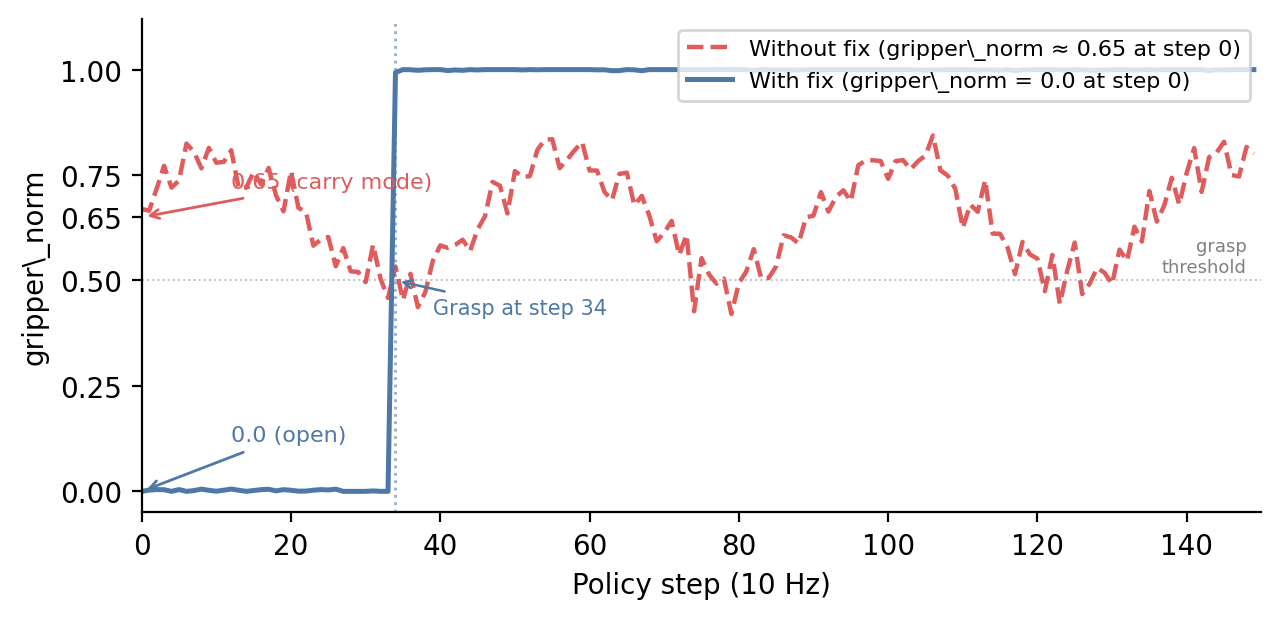
\includegraphics[width=\linewidth]{figures/04_gripper_init_fix.png}
\caption{Gripper initialisation mismatch: without the fix, the reset gripper control value ($\approx 0.65$) places the policy near the grasp threshold at step 0, causing spurious early carry-mode behaviour; resetting to fully open (0.0) restores the expected initial state.}
\label{fig:gripper_init_fix}
\end{figure}

\begin{figure}[H]
\centering
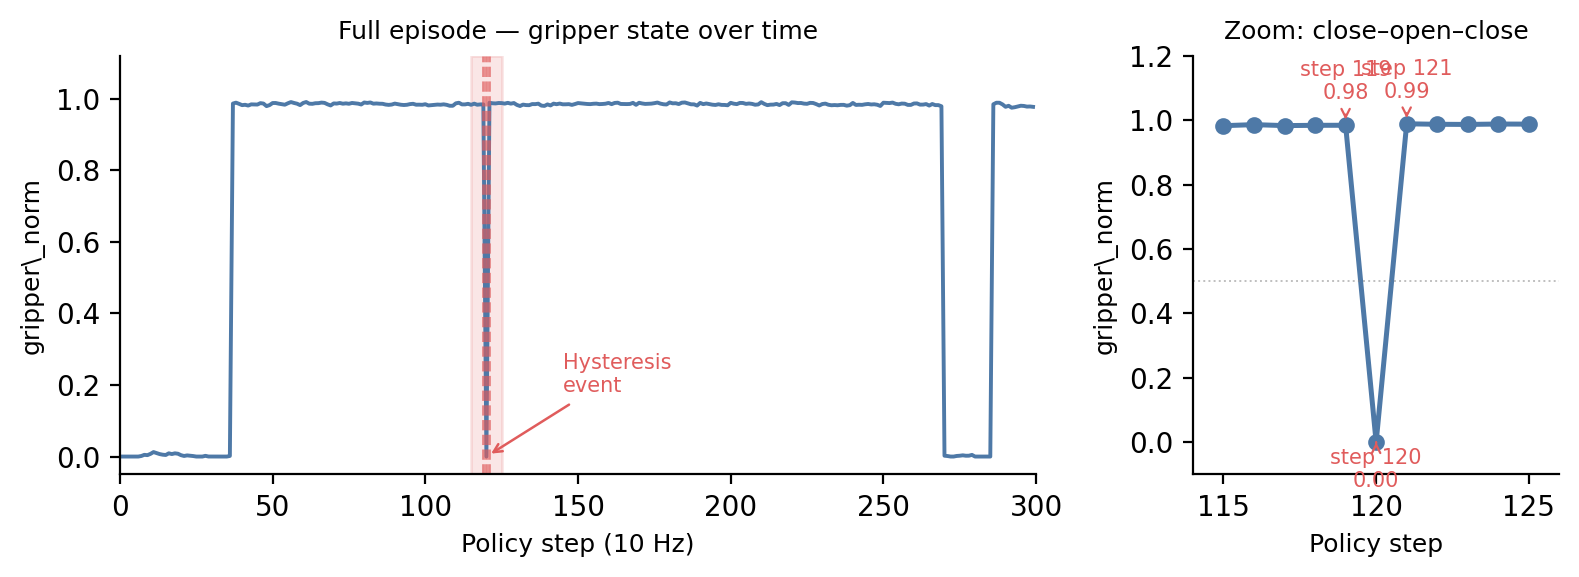
\includegraphics[width=\linewidth]{figures/06_gripper_hysteresis.png}
\caption{Gripper hysteresis: a spurious close--open--close event within a single action chunk (right, zoomed) would otherwise drop a carried object; the grasp-latch logic prevents this from reaching the gripper controller.}
\label{fig:gripper_hysteresis}
\end{figure}

These observations demonstrate that train--inference consistency is as important as the training configuration itself.

\subsubsection{Position-Control Policy Evaluation}

To address the limitations observed in velocity-control experiments, the action representation was redesigned to predict target joint positions rather than joint velocities. Under this formulation, a proportional controller converts predicted targets into executable velocity commands, separating the \emph{where} (learned by the policy) from the \emph{how fast} (handled by the controller). In practice, this produced smoother trajectories, more stable object approach motions, and more consistent grasp attempts. The \texttt{pos\_200k} checkpoint achieved 20\% trial-level success (12/60 trials) compared to 0\% for the velocity-control baseline, with the block-lifted rate rising from 0\% to 10--30\% across tasks that had previously shown no successful manipulation. Position-control policies were therefore adopted as the standard representation for all subsequent training runs.

\subsubsection{Checkpoint Comparison and Policy Evolution}

Five policy checkpoints were evaluated across the full six-task protocol (10 trials per task, 60 trials per checkpoint, except the velocity-control checkpoint which covers four tasks only). The checkpoints represent successive design iterations: \texttt{pi05\_base} (zero-shot), \texttt{vel\_100k} (100k steps, velocity control), \texttt{pos\_200k} (200k steps, position control), \texttt{pos\_v2} (500k steps, native 10\,Hz recording, 11-dim state), and \texttt{pos\_v3} (200k warm-start fine-tuning steps from \texttt{pos\_v2}, augmented near-side demonstrations); see Table~\ref{tab:checkpoints}.

\begin{table}[H]
\centering
\caption{Policy checkpoints evaluated throughout development.}
\label{tab:checkpoints}
\begin{tabularx}{\linewidth}{lllX}
\toprule
\textbf{Checkpoint} & \textbf{Steps} & \textbf{Key change} \\
\midrule
\texttt{pi05\_base} & --- & Zero-shot; no fine-tuning \\
\texttt{vel\_100k} & 100k & Velocity control; 4 tasks \\
\texttt{pos\_200k} & 200k & Position control; 6 tasks \\
\texttt{pos\_v2} & 500k & Native 10\,Hz; 11-dim state \\
\texttt{pos\_v3} & +200k & Warm-start v2; $\times$2.5 near demos \\
\bottomrule
\end{tabularx}
\par\footnotesize\emph{Note: 4 tasks = tasks with only red and blue blocks.}
\end{table}

\paragraph{Trial-level success rate.} Table~\ref{tab:trial_success} and Fig.~\ref{fig:success_bar_chart} report per-task trial-level success rates across all checkpoints. A trial is successful if the specified block reaches the correct side of the workspace divider ($x > 0.70$\,m for far; $x < 0.66$\,m for near).

\begin{table}[H]
\centering
\caption{Per-task trial-level success rate (successes / 10 trials). $\dagger$: green-block tasks were not in the velocity-control training set. Best-performing checkpoint shown in bold.}
\label{tab:trial_success}
\resizebox{\linewidth}{!}{%
\begin{tabular}{llccccc}
\toprule
\textbf{Task} & \textbf{Instruction} & \textbf{pi05\_base} & \textbf{vel 100k} & \textbf{pos 200k} & \textbf{pos\_v2} & \textbf{pos\_v3} \\
\midrule
T0 & Move red block $\to$ far & 7/10 & 0/10 & 1/10 & 6/10 & \textbf{9/10} \\
T1 & Move red block $\to$ near & 2/10 & 0/10 & 2/10 & 4/10 & \textbf{4/10} \\
T2 & Move blue block $\to$ far & 0/10 & 0/10 & 8/10 & 7/10 & \textbf{9/10} \\
T3 & Move blue block $\to$ near & 0/10 & 0/10 & 0/10 & \textbf{5/10} & 4/10 \\
T4 & Move green block $\to$ far & 0/10 & --$\dagger$ & 1/10 & \textbf{2/10} & 0/10 \\
T5 & Move green block $\to$ near & 0/10 & --$\dagger$ & 0/10 & 0/10 & 0/10 \\
\midrule
\textbf{Overall (trial-level)} & & 9/60 (15\%) & 0/40 (0\%) & 12/60 (20\%) & 24/60 (40\%) & \textbf{26/60 (43\%)} \\
\quad Far-side average & & 23\% & 0\% & 33\% & 50\% & \textbf{60\%} \\
\quad Near-side average & & 7\% & 0\% & 13\% & \textbf{30\%} & 27\% \\
\bottomrule
\end{tabular}%
}
\end{table}

\begin{figure}[H]
\centering
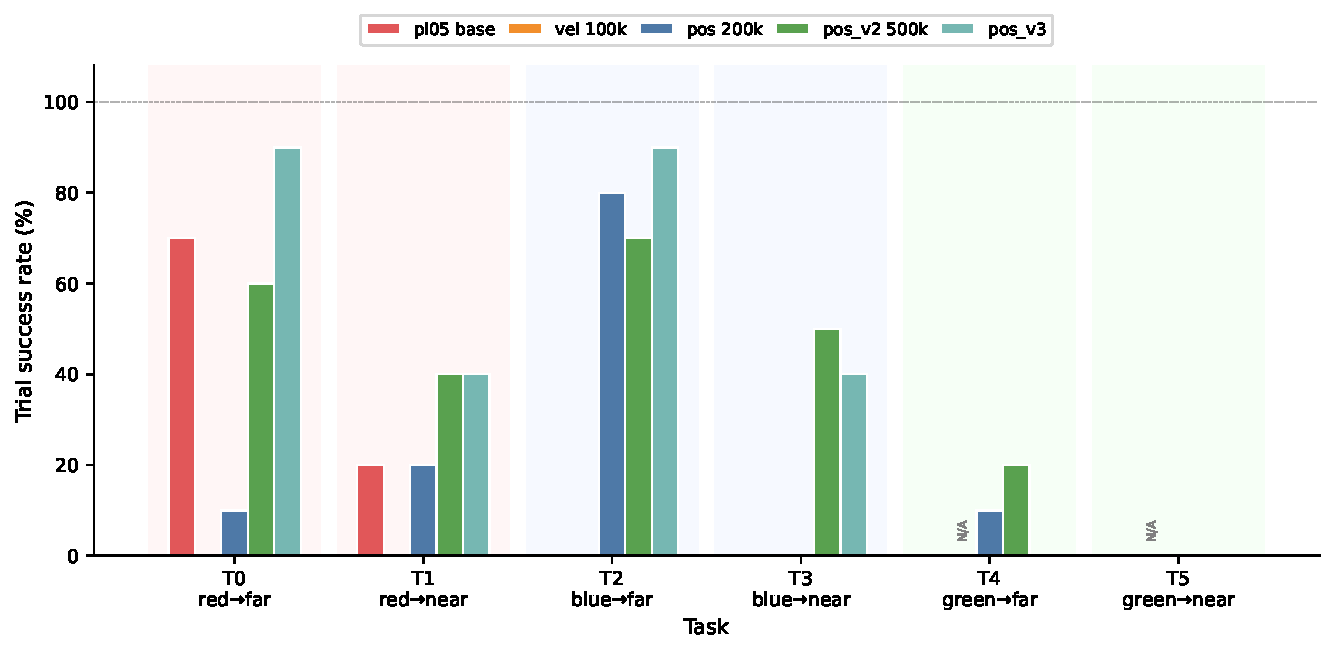
\includegraphics[width=\linewidth]{figures/late_stage_images/success_bar_chart.pdf}
\caption{Trial-level success rate by task and checkpoint (Table~\ref{tab:trial_success}), grouped by block colour.}
\label{fig:success_bar_chart}
\end{figure}

Several findings emerge from Table~\ref{tab:trial_success}. First, the zero-shot \texttt{pi05\_base} baseline achieves a non-trivial 15\% overall success rate (9/60 trials), with particularly strong performance on T0 (7/10, 70\% success). This result -- which contrasts with the na\"ive expectation that the pretrained model would entirely fail on an unseen embodiment -- confirms that $\pi$0.5 retains transferable manipulation priors, while also demonstrating that fine-tuning is necessary for reliable multi-task performance.

Second, a consistent far-side advantage is observed across all fine-tuned position-control checkpoints (far average: 20--60\%; near average: 7--30\%). Near-side carry requires the arm to move inward toward the robot base, which conflicts with the DLS null-space configuration and produces less consistent training demonstrations.

Third, green-block tasks (T4, T5) represent a persistent failure mode across all checkpoints, including \texttt{pos\_v3}, which was explicitly augmented with 250 near-side green demonstrations per task. The green block's position requires an arm configuration that approaches joint limits, and the \texttt{pos\_v3} checkpoint shows \emph{regression} on T4 (2/10 $\to$ 0/10) relative to \texttt{pos\_v2}, suggesting that the lower learning-rate warm-start did not provide sufficient gradient signal for this task. This is precisely the workspace-geometry effect that this final stage's cross-embodiment reach-margin methodology (Section~\ref{sec:methodology-crossemb}) was designed to characterise systematically on the new embodiments, isolating object location from training-data imbalance.

\paragraph{Manipulation quality: block-lifted rate.} Task success alone conflates true pick-and-place with accidental push success. Table~\ref{tab:lift_rate} disaggregates these by reporting the block-lifted rate, defined as the fraction of trials in which the block exceeded $z > 0.295$\,m, confirming a genuine grasp-and-lift occurred.

\begin{table}[H]
\centering
\caption{Block-lifted rate (\% of trials with block\_z $>$ 0.295\,m during the episode). Bold: highest per task.}
\label{tab:lift_rate}
\resizebox{\linewidth}{!}{%
\begin{tabular}{llccccc}
\toprule
\textbf{Task} & \textbf{Instruction} & \textbf{pi05\_base} & \textbf{vel 100k} & \textbf{pos 200k} & \textbf{pos\_v2 500k} & \textbf{pos\_v3} \\
\midrule
T0 & Move red block $\to$ far & 80\% & 0\% & 20\% & 70\% & \textbf{90\%} \\
T1 & Move red block $\to$ near & 20\% & 0\% & 30\% & 50\% & \textbf{70\%} \\
T2 & Move blue block $\to$ far & 0\% & 0\% & 30\% & \textbf{90\%} & 80\% \\
T3 & Move blue block $\to$ near & 0\% & 0\% & 30\% & \textbf{60\%} & 70\% \\
T4 & Move green block $\to$ far & 0\% & -- & 10\% & \textbf{30\%} & 0\% \\
T5 & Move green block $\to$ near & 0\% & -- & 10\% & \textbf{10\%} & 0\% \\
\midrule
\textbf{Mean lifted rate} & & 17\% & 0\% & 22\% & \textbf{50\%} & 45\% \\
\bottomrule
\end{tabular}%
}
\end{table}

Comparing Tables~\ref{tab:trial_success} and~\ref{tab:lift_rate} reveals an important discrepancy for \texttt{pos\_200k} at T2 (blue $\to$ far): 8/10 task-success but only 30\% lift rate, indicating that the majority of T2 successes were achieved through inadvertent pushing rather than controlled pick-and-place. Post-hoc grasp diagnostics confirmed a mean grasp error of $(-155, -78, -2)$\,mm for T2: the gripper closed 15.5\,cm laterally displaced from the block, and arm translation displaced the block to the far side. By contrast, \texttt{pos\_v2} achieves a lift rate well above its task-success rate for T2 (90\% lifted vs. 70\% success), confirming genuine pick-and-place. The \texttt{pos\_v3} checkpoint shows closer agreement between lift and success rates for blue tasks (80\% lifted vs. 90\% success on T2; 70\% vs. 40\% on T3), consistent with more reliable grasp execution overall.

\paragraph{Direction accuracy.} Table~\ref{tab:direction} reports the fraction of trials in which the block was displaced in the correct direction, regardless of whether the success threshold was crossed, measuring task understanding independently of execution precision.

\begin{table}[H]
\centering
\caption{Direction accuracy (\% of trials with correct-direction block displacement).}
\label{tab:direction}
\resizebox{\linewidth}{!}{%
\begin{tabular}{llccccc}
\toprule
\textbf{Task} & \textbf{Instruction} & \textbf{Base} & \textbf{Vel} & \textbf{Pos} & \textbf{V2} & \textbf{V3} \\
\midrule
T0 & Red $\to$ far & 100 & 0 & 50 & 100 & 100 \\
T1 & Red $\to$ near & 40 & 0 & 50 & 40 & 40 \\
T2 & Blue $\to$ far & 20 & 0 & 80 & 100 & 90 \\
T3 & Blue $\to$ near & 0 & 0 & 0 & 50 & 40 \\
T4 & Green $\to$ far & 10 & -- & 50 & 80 & 0 \\
T5 & Green $\to$ near & 0 & -- & 0 & 0 & 0 \\
\bottomrule
\end{tabular}%
}
\end{table}

Direction accuracy reveals task understanding not captured by binary success metrics. The \texttt{pos\_v2} checkpoint achieves 100\% direction accuracy on both T0 and T2 yet its task success on T4 remains only 20\%, confirming that the policy understands which direction to move for T4 but lacks the precision to cross the success threshold. By contrast, \texttt{pos\_v3} regresses to 0\% direction accuracy on T4, consistent with the collapsed prediction behaviour (arm hovering at pre-grasp for 600 steps) observed during diagnostic rollouts.

\paragraph{Training metrics and loss--performance relationship.} Table~\ref{tab:training_metrics} summarises the training configuration and final loss for each fine-tuned checkpoint. A key finding is that lower training loss does not correspond monotonically to improved task performance. The \texttt{pos\_v2} checkpoint achieves a final loss of 0.004 -- substantially lower than \texttt{pos\_200k} (0.008--0.015) -- yet achieves only marginal improvement in overall task success (40\% vs. 20\%). More strikingly, \texttt{pos\_v2} achieves fewer successes than \texttt{pos\_200k} on T2 (7/10 vs. 8/10) despite training 2.5$\times$ longer. These observations indicate that the primary bottleneck is not optimisation depth but the quality of training data (demonstration frequency, state representation, and grasp precision); the introduction of native 10\,Hz demonstration recording and end-effector Cartesian coordinates in \texttt{pos\_v2} had a greater qualitative effect on lifting behaviour (mean lifted rate 50\% vs. 22\%) than on raw task success.

\begin{table}[H]
\centering
\caption{Training configuration and final metrics for each fine-tuned checkpoint.}
\label{tab:training_metrics}
\begin{tabular}{lccccc}
\toprule
\textbf{Config} & \textbf{Steps} & \textbf{Demos} & \textbf{State} & \textbf{Loss} \\
\midrule
vel & 100k & 400 & 8D & -- \\
pos & 200k & 600 & 8D & 0.008--0.015 \\
pos\_v2 & 500k & 600 & 11D & 0.004 \\
pos\_v3 & +200k & 950 & 11D & $<$0.004 \\
\bottomrule
\end{tabular}
\par\footnotesize\emph{Note: all checkpoints used a peak learning rate of $2\times10^{-4}$ except \texttt{pos\_v3}, which used $5\times10^{-5}$.}
\end{table}

\paragraph{Failure mode analysis.} Analysis of policy rollouts identified grasp precision as the dominant remaining failure mode. Although the policy consistently selected the correct object and generated appropriate approach trajectories, small spatial errors during gripper alignment frequently prevented successful object pickup. Additional failures included premature gripper release during transport and occasional policy collapse, in which the robot remained near the pre-grasp pose throughout the episode. An important secondary observation was the difference in performance between workspace regions: tasks requiring movement towards the far side consistently achieved higher success rates than equivalent near-side tasks, suggesting that the latter were underrepresented in the training data or more difficult to execute due to workspace geometry.

\paragraph{Zero-shot baseline analysis.} The \texttt{pi05\_base} zero-shot result (15\% overall success, 7/10 on T0) is consistent with $\pi$0.5's pretraining on large-scale, diverse robot manipulation data: the model's pretrained manipulation priors partially generalise to the Baxter workspace and camera configuration, achieving an 80\% block-lift rate and 100\% direction accuracy on T0. The performance collapse on blue and green blocks (0/10 success, near-zero lift rates) demonstrates the limits of zero-shot generalisation: the pretrained model cannot reliably distinguish between the three block colours from the current camera viewpoint, defaulting to the dominant pretraining behaviour of approaching objects in the centre of the scene, which corresponds to the red block's position. This motivates fine-tuning as a mechanism not only for embodiment adaptation but for task routing across multiple objects with distinct spatial locations.

This zero-shot result also usefully calibrates how the checkpoint comparison in Table~\ref{tab:trial_success} should be read. Because \texttt{pi05\_base} already succeeds on 70\% of T0 trials without any Baxter-specific data at all, the improvement from \texttt{pi05\_base} to \texttt{pos\_v3} on T0 (70\% to 90\%) is a considerably smaller relative gain than the improvement on T2 (0\% to 90\%), even though both reach a similar final success rate. Fine-tuning's measurable contribution is therefore concentrated almost entirely in tasks where the pretrained model's zero-shot priors do not already transfer -- blue and green blocks -- rather than being evenly distributed across all six tasks, which is consistent with the account above of zero-shot performance being governed by which object happens to sit where the pretrained model already expects to find something.

\begin{figure}[H]
\centering
\begin{subfigure}[b]{0.32\linewidth}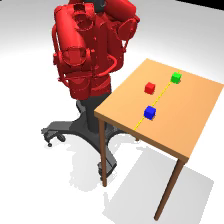
\includegraphics[width=\linewidth]{figures/late_stage_images/a_initial.png}\caption{Initial}\end{subfigure}
\begin{subfigure}[b]{0.32\linewidth}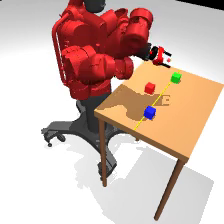
\includegraphics[width=\linewidth]{figures/late_stage_images/b_approach.png}\caption{Approach}\end{subfigure}
\begin{subfigure}[b]{0.32\linewidth}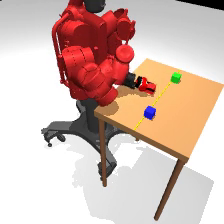
\includegraphics[width=\linewidth]{figures/late_stage_images/c_descent.png}\caption{Descent}\end{subfigure}

\begin{subfigure}[b]{0.32\linewidth}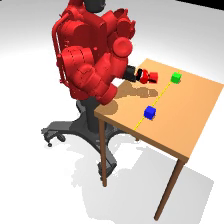
\includegraphics[width=\linewidth]{figures/late_stage_images/d_lift.png}\caption{Lift ($z=0.35$\,m)}\end{subfigure}
\begin{subfigure}[b]{0.32\linewidth}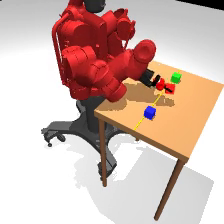
\includegraphics[width=\linewidth]{figures/late_stage_images/e_carry.png}\caption{Carry ($x=0.75$\,m)}\end{subfigure}
\begin{subfigure}[b]{0.32\linewidth}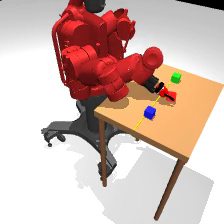
\includegraphics[width=\linewidth]{figures/late_stage_images/f_place.png}\caption{Place ($x=0.76$\,m)}\end{subfigure}
\caption{Execution sequence for a successful red-block far-side trial (\texttt{pos\_v3}, T0, trial 00, 9/10 success rate). The policy executes a complete pick-and-place sequence: approach, descent to within 3\,mm of block centre, lift to 0.37\,m, carry across the workspace divider, and controlled placement. Final block position: $x = 0.779$\,m (success threshold: $x > 0.70$\,m).}
\label{fig:exec_sequence}
\end{figure}

Fig.~\ref{fig:exec_sequence} shows the full six-frame execution sequence of a representative successful trial, illustrating what this pick-and-place structure looks like when execution is precise. Overall, this failure analysis indicates that the policy has learned the high-level structure of the manipulation task but remains limited by execution accuracy rather than task understanding.

\subsection{VLM Planner Evaluation}
\label{sec:results-vlm}

The planner's implementation (Section~\ref{sec:vlm-planner}) has been exercised qualitatively throughout development: the per-block prompting strategy, the goal-check query, and the full plan--execute--check loop run end-to-end against the MuJoCo simulation, correctly identifying which of the three blocks require movement and generating a syntactically valid, executable task list for representative current/goal image pairs inspected during development (Fig.~\ref{fig:vlm_pipeline}, Fig.~\ref{fig:goal_grid}).

A quantitative evaluation protocol, following directly from the evaluation methodology in Section~\ref{sec:methodology}, is defined but not yet executed at the time of writing: (i) \emph{position-classification accuracy} -- for each of the 8 goal configurations and a matched set of initial configurations, the fraction of per-block current/goal position queries the planner answers correctly against ground truth; (ii) \emph{task-list correctness} -- whether the resulting primitive list, compared against an oracle list computed directly from the known block positions, is both minimal (no unnecessary primitives for blocks already at their goal position) and complete (no missing primitives); and (iii) an \emph{oracle-ordering ablation}, in which the policy is driven by the oracle task list rather than the VLM-planned list, isolating planning errors from policy-execution errors in the resulting collaborative task success rate reported in Section~\ref{sec:results-hrc}. Running this evaluation across all 8 goal configurations, with repeated trials per configuration to account for the planner's non-deterministic image-conditioned reasoning, is the immediate next step before the collective-task evaluation of Section~\ref{sec:results-hrc} can be interpreted with planning and execution error attributed correctly. A minimum of five repeated queries per block per configuration (120 queries in total across the 8-configuration goal space) is planned, sufficient to distinguish a systematic per-colour misclassification from occasional single-query noise given the qualitative reliability already observed during development; this sample size can be revisited once the first batch of results is available.

\subsection{Cross-Embodiment Generalisability}
\label{sec:results-crossemb}

\subsubsection{Demonstration Collection Results}
Data collection for both new embodiments is complete. Episode counts per task were scaled to observed yield from small-batch pilot tests, oversampling low-yield tasks, following the same oversample-and-filter approach already used for the Baxter dataset. Table~\ref{tab:franka_yield} and Table~\ref{tab:g1_yield} report the resulting yields, for the scenes shown in Fig.~\ref{fig:cross_embodiment_scenes}.

\begin{table}[H]
\centering
\caption{Franka demonstration collection yield (\texttt{data/pickplace\_franka\_pos/}).}
\label{tab:franka_yield}
\begin{tabular}{lccc}
\toprule
\textbf{Task} & \textbf{Attempted} & \textbf{Successful} & \textbf{Yield} \\
\midrule
0: red $\to$ far & 30 & 28 & 93.3\% \\
1: red $\to$ near & 30 & 27 & 90.0\% \\
2: blue $\to$ far & 40 & 17 & 42.5\% \\
3: blue $\to$ near & 40 & 29 & 72.5\% \\
4: green $\to$ far & 100 & 25 & 25.0\% \\
5: green $\to$ near & 60 & 2 & 3.3\% \\
\midrule
\textbf{Total} & 300 & \textbf{128} & 42.7\% \\
\bottomrule
\end{tabular}
\end{table}

\begin{table}[H]
\centering
\caption{G1 demonstration collection yield (\texttt{data/pickplace\_g1\_pos/}). Tasks 3 and 5 excluded -- 0\% yield at pilot scale, a reach-envelope limit rather than a bug.}
\label{tab:g1_yield}
\begin{tabular}{lccc}
\toprule
\textbf{Task} & \textbf{Attempted} & \textbf{Successful} & \textbf{Yield} \\
\midrule
0: red $\to$ far & 30 & 30 & 100\% \\
1: red $\to$ near & 30 & 30 & 100\% \\
2: blue $\to$ far & 30 & 30 & 100\% \\
4: green $\to$ far & 30 & 23 & 76.7\% \\
\midrule
\textbf{Total} & 120 & \textbf{113} & 94.2\% \\
\bottomrule
\end{tabular}
\end{table}

128 successful Franka episodes (22{,}076 frames) and 113 successful G1 episodes (10{,}867 frames) were converted to the LeRobot format and verified to match the Baxter dataset's schema exactly. G1's excluded tasks (blue-near, green-near) reflect a genuine, position-dependent reach-margin trade-off of the shorter G1 arm at its current base position, confirmed by testing three candidate base positions and selecting the best overall trade-off (Section~\ref{sec:methodology-crossemb}), rather than an unresolved bug. Franka's green-near task, while technically included (2/60 successful episodes), is too thin to be meaningful on its own and is flagged as such rather than silently included at full weight.

The two embodiments show markedly different overall yield profiles -- 42.7\% for Franka versus 94.2\% for G1 -- which is informative in its own right rather than simply a measure of which embodiment is ``easier''. G1's yield is high but over a narrower effective task set (four of six tasks attempted at production scale, per Section~\ref{sec:methodology-crossemb}'s reach-margin finding), while Franka's yield is lower but spans all six tasks, concentrated specifically in the two tasks requiring the longest reach (green-far at 25.0\% and green-near at 3.3\%), consistent with the base-position reach analysis in Section~\ref{sec:crossemb-bugs} rather than a uniform degradation across tasks. Put differently, both embodiments' shortfalls are explained by the same underlying cause -- a fixed base position trading off reach margin against different corners of the shared workspace -- rather than by two unrelated embodiment-specific weaknesses, which is itself a mildly encouraging sign for the joint cross-embodiment training in Section~\ref{sec:methodology-crossemb}: the failure modes are geometric and per-task rather than idiosyncratic to either robot's control interface, so they are not obviously the kind of thing that would be expected to interfere destructively with a jointly trained policy's shared representation, though this remains to be confirmed once training is run.

\subsubsection{Training and Transfer Evaluation}
The joint mixture-loading training configuration (Section~\ref{sec:methodology-crossemb}) has been mechanically validated -- the configuration loads, and the data loader produces correctly normalised, correctly mixed batches across all three embodiments -- but no training run has yet been launched. The solo-versus-joint comparison that constitutes the actual test of RQ4 therefore requires three further training runs: \texttt{pi05\_franka\_pickplace\_pos} and \texttt{pi05\_g1\_pickplace\_pos} trained independently as solo baselines (reusing the existing, already-validated Baxter \texttt{pos\_v3} run as the Baxter solo baseline), and \texttt{pi05\_cross\_embodiment\_pickplace} trained jointly across all three datasets with the current equal mixture weighting. None of these runs have started at the time of writing; launching them, and evaluating each resulting policy using the same trial-level, block-lifted, and direction-accuracy metrics used for Baxter in Section~\ref{sec:results-sim}, per embodiment, is the immediate next step for this experiment.

\subsection{Human-Robot Collaboration: Collective Task}
\label{sec:results-hrc}

The collective-task evaluation protocol defined in Section~\ref{sec:methodology-hrc} has not yet been run. The supporting infrastructure -- the VLM planner's closed-loop goal-check--replan cycle (Section~\ref{sec:vlm-planner}) and the \texttt{SimRunner} integration executing planner-issued primitives sequentially against the fine-tuned policy -- is implemented and has been exercised for planner-only and single-primitive execution during development, but trials combining a human-modified initial configuration, multi-primitive execution, and a mid-execution human intervention have not yet been conducted. Collecting these trials, across a representative sample of the 8-configuration goal space (Fig.~\ref{fig:goal_grid}) and a range of intervention timings, and reporting collaborative task success alongside the replanning-trigger and replanning-correctness metrics defined in Section~\ref{sec:methodology-hrc}, is the primary remaining evaluation for this dissertation. The planned trial matrix covers each of the 8 goal configurations under three conditions -- no intervention, an early intervention (before the first primitive completes), and a late intervention (after most primitives have completed) -- giving 24 trials as an initial target, sized to be large enough to distinguish a systematic replanning failure from an isolated one while remaining feasible within a single supervised session per configuration set, given that each trial requires a human physically present to place and, where applicable, reposition blocks.

\subsection{Real Robot Validation}
\label{sec:results-realrobot}

The real-robot deployment architecture described in Section~\ref{sec:methodology-realrobot} -- the ROS-based robot client, the RealSense-camera-injecting policy server wrapper, and the shared P-controller and grasp-latch logic -- is implemented. At the time of writing, this deployment has not yet been exercised end-to-end on the physical Baxter robot: the single-block pick-and-place validation trial (task~0) described in Section~\ref{sec:methodology-realrobot} is scheduled as the first physical evaluation, to be followed by extension to the full six-primitive set if successful. No sim-to-real success-rate comparison is therefore yet available; this is reported as the outstanding item most directly tied to RQ6. Once run, the single-block trial will be evaluated under the identical 10-trial, trial-level success protocol used for every simulation checkpoint in Table~\ref{tab:trial_success}, so that the resulting physical success rate is directly comparable, trial-for-trial, against \texttt{pos\_v3}'s 9/10 simulation result on the same task, rather than requiring a separate bespoke metric to be defined for the physical robot.

Should the single-block trial succeed at a rate broadly comparable to simulation, the planned extension is to progress through the remaining five primitives individually (T1--T5 of Table~\ref{tab:trial_success}), in the same order of simulation difficulty already established -- far-side tasks before near-side tasks, red and blue blocks before the persistently harder green block -- so that any physical-only failure mode is first isolated on the tasks most likely to succeed, rather than risking an early, uninformative failure on the hardest simulation task (green-near, 0\% success even in simulation) before the sim-to-real gap on the easier tasks has been established. Only once all six primitives have been individually validated would the full VLM-planner-driven multi-primitive sequences of Section~\ref{sec:vlm-planner} be attempted on the physical robot, deliberately mirroring the same staged, single-component-before-integration approach used throughout this project (Section~\ref{sec:design-approach}).

% =====================================================================
\section{Discussion and Critical Reflection}
\label{sec:discussion}

\subsection{Evaluation of Research Progress}

Across the three stages of this project, the core technical objectives established at the early-stage gateway have been completed: a simulation environment, a scripted demonstration-collection pipeline, LoRA-based VLA adaptation, redesign of the action representation from velocity to position control, and a Vision--Language planner with a working closed-loop re-planning mechanism. This final stage's three new lines of work -- cross-embodiment extension, the collective-task protocol, and real-robot deployment infrastructure -- are each at a different point of completion: cross-embodiment data collection is finished and joint training is mechanically validated but not yet run; the collective-task protocol and its supporting closed-loop mechanism are fully specified and implemented but not yet exercised as trials; and real-robot deployment infrastructure is implemented but not yet exercised on hardware at all. This uneven state of completion is itself informative: it reflects that data collection and infrastructure engineering, which are largely mechanical once the underlying pipeline exists, complete faster than the evaluation trials that depend on GPU-hours (training runs) or coordinated human-in-the-loop sessions (the collective task), which are the genuine remaining bottleneck for this dissertation.

Against the specific research questions posed in Section~\ref{sec:gap}, this leaves RQ1--RQ3 answered with completed quantitative evidence, and RQ4--RQ6 answered at the level of implemented, validated infrastructure and a fully specified evaluation protocol, but not yet at the level of the quantitative result each question ultimately asks for. This is a materially different, and more advanced, state of progress than at the late-stage gateway, where the corresponding future-work items (human-robot collaboration evaluation, physical deployment) existed only as stated intentions with no supporting implementation; the remaining task before final submission is therefore one of running already-built experiments and reporting their results, rather than of designing or implementing new system components.

\subsection{Comparison to Related Systems}

It is useful to place the completed system against the closest related work identified in Section~\ref{sec:litrev}. VLA-bot combines multimodal perception with manipulation for collaborative assembly, but requests human assistance through an augmented-reality interface and relies on a custom, task-specific mapping from human input to motion sequences rather than a large pretrained VLA policy \cite{WANG2026103268}; the system reported here instead uses a foundation-scale, pretrained-then-fine-tuned VLA policy throughout, and requests human involvement only implicitly, through the collective task's shared workspace, rather than through an explicit assistance-request interface. Wang~\emph{et al.}'s bidirectional communication framework allows a human to modify a robot's trajectory in real time via natural language \cite{wang2026bidirectionalhumanrobotcommunicationphysical}, but modifies a trajectory that is otherwise predefined; the VLM planner's closed-loop re-planning (Section~\ref{sec:vlm-planner}) instead regenerates the entire remaining task sequence from a re-observed scene, which is a coarser-grained but more scene-grounded form of adaptation -- it responds to what has physically changed in the workspace rather than to an explicit verbal correction, which is precisely what the collective task's mid-execution intervention is designed to exercise. Neither comparator system reports adapting its action-generation component to more than one robot embodiment, which remains, so far as this literature review found, a genuine point of distinction for the cross-embodiment extension in Section~\ref{sec:methodology-crossemb}.

\subsection{Methodological Reflection}

The simulation-first development strategy, adopted from the outset, continued to prove valuable in this final stage: constructing the Franka and G1 scenes and demonstration pipelines in simulation before any hardware was acquired allowed the reach-margin methodology (Section~\ref{sec:methodology-crossemb}) to be developed and applied twice, cheaply, before either new embodiment's dataset was finalised, in a way that would have been prohibitively slow with physical robots. The same iterative, checkpoint-driven development process used for the Baxter policy -- evaluate, diagnose, fix, re-evaluate -- was reused directly for diagnosing the cross-embodiment bugs recorded in the accompanying engineering log, each traced to a specific, previously enumerated cause (self-collision, home-pose transit height, IK instability at a joint limit, insufficient gripper force, block slip on release) rather than treated as an unexplained embodiment difference.

A specific methodological contribution of this final stage is the per-block VLM prompting strategy (Section~\ref{sec:vlm-planner}), which directly resolves a limitation identified during the \emph{early} stage of the project (Section~\ref{sec:early-monitoring}): that Gemma-3-12B produced accurate free-form scene descriptions but unreliable structured output when reasoning about multiple objects at once. Rather than attempting to improve the model's multi-object reasoning directly, the planner sidesteps the problem by construction -- one object, one tightly scoped, fixed-format question at a time -- which is a general pattern likely applicable beyond this project wherever a VLM is used for structured, multi-entity scene monitoring.

A limitation of the methodology as a whole, acknowledged already at the late stage and only partially addressed here, is that evaluation has been conducted almost entirely within simulation; the real-robot deployment architecture in Section~\ref{sec:methodology-realrobot} is designed specifically to close this gap, but its results are not yet available. Consequently, the reported findings continue to demonstrate feasibility within simulation and via mechanically validated, but not yet executed, extensions, rather than fully closing the loop on physical hardware.

A related, narrower limitation concerns the scope of the manipulation task itself: all quantitative results in this dissertation, across all three embodiments, concern a single class of task -- moving one of three coloured blocks between two workspace regions -- and it is not established how far the specific findings (for example, the far-side advantage, or the green-block failure mode of Section~\ref{sec:results-sim}) generalise beyond this task family to substantially different manipulation tasks (stacking, insertion, or tasks involving deformable or articulated objects). The task decomposition into six reusable primitives (Section~\ref{sec:demo-pipeline}) was a deliberate simplification to make policy learning and planner integration tractable within an MRes timeline, and the finding that this decomposition transferred cleanly to two further embodiments (Section~\ref{sec:methodology-crossemb}) is evidence that the decomposition itself is a reasonable one, but it does not by itself establish that the underlying engineering lessons -- on action representation, train--inference consistency, or per-block VLM prompting -- would transfer unchanged to a task family with materially different contact dynamics or a larger action vocabulary.

\subsection{Lessons Learned}

The most important lesson from the late stage -- that successful adaptation of Vision-Language-Action models depends more on system design than optimisation alone -- was reconfirmed by this final stage's checkpoint findings (Section~\ref{sec:results-sim}) and extended by the cross-embodiment work: improvements in manipulation performance were driven primarily by changes to the action representation and train--inference consistency rather than by longer training or lower loss, and the same held true for demonstration quality across the two new embodiments, where over-recording and success-filtering, rather than any change to the underlying DLS controller, was what made the Franka and G1 datasets usable.

A second lesson, specific to this final stage, is that decomposing the manipulation task into six reusable primitives -- a decision made early in the late stage to simplify policy learning and planner integration -- turned out to generalise cleanly to entirely new embodiments as well: the same task set, the same primitive vocabulary, and the same DLS controller mathematics transferred to Franka and G1 with only the per-embodiment kinematic chain and reach margins needing to change. This suggests that a well-chosen task decomposition is a reusable design asset that pays off beyond its original scope.

Finally, engineering the VLM planner's structured-output reliability and its closed-loop re-planning cycle before attempting the collective-task trials, rather than the reverse, proved to be the right ordering: the per-block prompting fix and the goal-check mechanism are prerequisites for the collective task producing an interpretable result at all, since a failed collective-task trial would otherwise be difficult to attribute to planning error, policy execution error, or the human's own actions.

A fourth, more general lesson from this final stage is that infrastructure work and evaluation work have very different, and easy-to-conflate, notions of ``done''. Cross-embodiment data collection, the collective-task closed-loop mechanism, and the real-robot client/server pair are all complete in the sense that the code runs, produces the expected intermediate artefacts, and has been exercised qualitatively -- yet none of them yet answers the research question it was built to answer, because none of the three comparison experiments (solo-versus-joint training, intervention trials, sim-to-real trials) has actually been run. Recognising this distinction explicitly, rather than reporting infrastructure completion as if it were equivalent to a completed experiment, is itself a methodological discipline worth naming, and is why Sections~\ref{sec:results-crossemb}--\ref{sec:results-realrobot} are written the way they are: as an honest account of what has and has not yet been measured, rather than as results sections padded with implementation detail in place of findings.

\subsection{Ethical and Practical Considerations for Deployment}

Human--robot collaboration systems of the kind proposed here must consider user trust, physical safety, and interaction quality, a point raised already at the early-stage gateway but only lightly addressed since the system evaluated at that stage did not yet involve a human sharing a workspace with a moving robot arm. This final stage's collective-task protocol (Section~\ref{sec:methodology-hrc}) and physical deployment (Section~\ref{sec:methodology-realrobot}) make these considerations concrete rather than abstract. Physically, the velocity and command-timeout limits described in Section~\ref{sec:methodology-realrobot} are safety-relevant, not merely functional: a $1.5$\,rad/s joint-velocity limit and a reliable Ctrl-C stop path are minimum requirements before a human is asked to stand at the same workspace the arm is moving in, and any collective-task trial involving a human physically repositioning blocks while the arm is active should extend these with a workspace boundary or supervised e-stop rather than relying on the velocity limit alone. From a trust perspective, the collective task's closed-loop re-planning (Section~\ref{sec:vlm-planner}) means the robot's next action is not always predictable to a human partner from the immediately preceding one, since it depends on a VLM's re-interpretation of the scene; the replanning-correctness metric proposed in Section~\ref{sec:methodology-hrc} is therefore also, in effect, a proxy for how predictable -- and hence how trustworthy -- the system would appear to a human collaborator, and should be reported alongside, not only as a supplement to, raw collaborative task success.

\subsection{Reproducibility}

Throughout this project, an emphasis was placed on keeping the pipeline reproducible rather than relying on manually tuned, one-off runs. Every reported checkpoint (Table~\ref{tab:checkpoints}) is tied to a fixed, versioned demonstration dataset and a specific training configuration (Table~\ref{tab:training_metrics}); the scripted, IK-based demonstration generation used throughout (Section~\ref{sec:demo-pipeline}) means any dataset can, in principle, be regenerated from the same scene definition and task parameters rather than depending on unrepeatable human teleoperation. The same applies to the cross-embodiment extension, where the reach-margin methodology of Section~\ref{sec:methodology-crossemb} was deliberately written up as a general, repeatable diagnostic procedure rather than a one-off fix, precisely so that it could be, and was, applied a second time to G1 after first being developed for Franka. Project updates, demonstration videos, and source code are made available at the repository referenced in the abstract, and the accompanying engineering log documenting every bug and fix encountered during the cross-embodiment extension (referenced throughout Section~\ref{sec:methodology-crossemb}) is maintained as a standing artefact alongside the code, so that the specific cause of each resolved issue remains traceable rather than only its final fix.

% =====================================================================
\section{Conclusion and Future Work}
\label{sec:conclusion}

This dissertation has presented the complete arc of an MRes project adapting the $\pi$0.5 Vision--Language--Action model to a Baxter-based human-robot collaboration system, from an early-stage exploration of vision--language monitoring and a first, informative zero-shot failure, through a late-stage fine-tuning and inference pipeline that improved trial-level manipulation success from 0\% to 43\% across six tasks, to this final stage's three extensions: cross-embodiment generalisation to Franka and G1, a substantially expanded and now closed-loop Vision--Language planner with a defined collective-task evaluation protocol, and infrastructure for validating the fine-tuned policy on a physical Baxter robot.

Restated against the six research questions posed in Section~\ref{sec:gap}, this dissertation's findings are:
\begin{itemize}[nosep]
\item \textbf{RQ1--RQ2} (embodiment adaptation and engineering decisions): a pretrained $\pi$0.5 policy transfers partially but unreliably to a novel Baxter embodiment zero-shot (15\% success), and LoRA fine-tuning combined with a position-control action representation and systematic elimination of train--inference mismatches raises this to 43\% trial-level success across six tasks -- answered in full, in Section~\ref{sec:results-sim}.
\item \textbf{RQ3} (planner--policy integration): a Gemma-3-12B VLM planner, using per-block constrained-format prompting to work around known multi-object structured-output unreliability, successfully decomposes goal images into primitive sequences and closes the loop with a goal-check--replan cycle -- implemented and qualitatively validated in Section~\ref{sec:vlm-planner}, with quantitative planning accuracy pending (Section~\ref{sec:results-vlm}).
\item \textbf{RQ4} (cross-embodiment transfer): demonstration collection for Franka and G1 is complete (128 and 113 episodes respectively) and joint-mixture training is mechanically validated, but the solo-versus-joint training comparison that would answer this question has not yet been run (Section~\ref{sec:results-crossemb}).
\item \textbf{RQ5} (collective task): the evaluation protocol and its supporting closed-loop infrastructure are fully specified and implemented, but no collective-task trials have yet been conducted (Section~\ref{sec:results-hrc}).
\item \textbf{RQ6} (sim-to-real transfer): the physical deployment architecture is implemented but not yet exercised on the physical robot, so the sim-to-real gap remains unmeasured (Section~\ref{sec:results-realrobot}).
\end{itemize}

The immediate remaining work, in priority order, is: (1) launching the three cross-embodiment training runs (Franka solo, G1 solo, and the joint mixture policy) and evaluating positive or negative skill transfer against the existing Baxter baseline; (2) executing the VLM planner's quantitative evaluation protocol, including the oracle-ordering ablation, to establish planning accuracy independently of policy execution; (3) running the collective-task trials, including human mid-execution interventions, to report the collaborative task success metric defined in this dissertation; and (4) exercising the real-robot deployment on the physical Baxter robot, beginning with the single-block validation trial and extending to the full task set if successful, to finally answer the sim-to-real question raised throughout this work.

Together, the completed and in-progress work reported here demonstrates that adapting a foundation-scale VLA model to a novel robot embodiment is achievable with modest fine-tuning data given careful attention to action representation and train--inference consistency; that a VLM planner can be engineered around known multi-object reasoning weaknesses to reliably decompose and monitor goal-directed rearrangement; and that the same pipeline extends, with largely mechanical effort, to further embodiments and to physical hardware, positioning the project well for a complete, evaluated human-robot collaboration system by final submission.

More broadly, the trajectory of this project across its three stages -- from an early-stage pilot that deliberately tested two competing monitoring strategies against each other, through a late-stage programme that isolated action representation and train--inference consistency as the dominant levers on manipulation performance, to this final stage's three-pronged extension into cross-embodiment transfer, closed-loop collaboration, and physical deployment -- illustrates a broader claim about how foundation-scale robot learning models should be adapted in practice: not by treating the pretrained model as a black box to be fine-tuned once and deployed, but by treating adaptation itself as an engineering process with identifiable failure modes, each diagnosable and fixable in isolation, whether that failure mode concerns a mismatched action space, an unreliable VLM output format, or a robot-specific reach margin. The remaining work identified above is substantial, but it is work of a different, more tractable kind than what preceded it: running and reporting on infrastructure and protocols that are already built, rather than designing, building, or debugging new ones.

% =====================================================================
\section{Acknowledgement of AI Usage}

This dissertation was developed with the assistance of AI tools (Claude Code) for drafting, restructuring, and LaTeX editing, working from the author's own early- and late-stage report drafts, experimental logs, and source code. All experimental work, results, engineering decisions, and critical analysis presented in this dissertation are the author's own; sections describing experiments not yet completed at the time of writing are explicitly marked as such rather than presented as completed findings. The use of AI tools was limited to enhancing productivity and readability, and all outputs were carefully reviewed and validated against the underlying reports, logs, and code before inclusion.

\clearpage
\bibliographystyle{IEEEtran}
\bibliography{references}

\end{document}
